\documentclass[11pt, a4paper]{article}

% --- 1. GEOMETRÍA Y MÁRGENES ---
\usepackage[
    a4paper,
    left=2cm, right=2cm,
    top=1.2cm, bottom=2.0cm,
    includehead, headheight=105pt, headsep=0.5cm
]{geometry}

\usepackage[spanish,es-tabla,es-nodecimaldot]{babel}
\usepackage{fontspec}
\setmainfont{texgyretermes}[Extension=.otf, UprightFont=*-regular, BoldFont=*-bold, ItalicFont=*-italic, BoldItalicFont=*-bolditalic]
\setmonofont{DejaVuSansMono}[Extension=.ttf, BoldFont=*-Bold, ItalicFont=*-Oblique, BoldItalicFont=*-BoldOblique, Scale=0.84]
\usepackage{newunicodechar}
\newunicodechar{→}{\ensuremath{\rightarrow}}
\newunicodechar{−}{\ensuremath{-}}
\newunicodechar{≥}{\ensuremath{\geq}}
\newunicodechar{≤}{\ensuremath{\leq}}
\usepackage{microtype}
\usepackage{xurl}
\usepackage{graphicx}
\usepackage{fancyhdr}
\usepackage{xcolor}
\usepackage{colortbl}
\usepackage{tabularx}
\usepackage{longtable}
\usepackage{array}
\usepackage{setspace}
\usepackage{enumitem}
\usepackage{lastpage}
\usepackage{float}
\usepackage{needspace}
\usepackage[section]{placeins}
\usepackage{caption}
\usepackage{multirow}
\usepackage{amsmath}
\usepackage{amssymb}
\usepackage[
    colorlinks=true,
    urlcolor=colabpyblue,
    linkcolor=colabpyblue,
    citecolor=colabpyblue,
    breaklinks=true
]{hyperref}

% --- 2. LIBRERÍAS DE DISEÑO AVANZADO ---
\usepackage[most]{tcolorbox}
\tcbuselibrary{listings, skins, breakable}
\usepackage{fontawesome5}
\usepackage{pifont}
\usepackage{listings}

% --- 3. PALETA DE COLORES INSTITUCIONALES (UNSA) ---
\definecolor{unsared}{RGB}{230, 25, 45}
\definecolor{colabpyblue}{RGB}{25, 55, 90}
\definecolor{colabpybg}{RGB}{242, 247, 252}
\definecolor{colaboutgreen}{RGB}{45, 90, 60}
\definecolor{colaboutbg}{RGB}{245, 252, 245}
\definecolor{tableheader}{RGB}{242, 242, 242}
\definecolor{checkgreen}{RGB}{34, 139, 34}
\definecolor{codegray}{RGB}{248, 248, 248}
\definecolor{codecomment}{RGB}{110, 110, 110}
\definecolor{codestring}{RGB}{163, 21, 21}
\definecolor{codekeyword}{RGB}{25, 55, 160}

\emergencystretch=3em
\captionsetup{font=small, labelfont=bf, labelsep=period}
\renewcommand{\topfraction}{0.9}\renewcommand{\bottomfraction}{0.8}\renewcommand{\textfraction}{0.08}\renewcommand{\floatpagefraction}{0.75}\setcounter{topnumber}{3}\setcounter{totalnumber}{4}
\captionsetup[table]{position=top, skip=4pt}
\renewcommand{\listfigurename}{\textcolor{colabpyblue}{Índice de Figuras}}
\renewcommand{\listtablename}{\textcolor{colabpyblue}{Índice de Tablas}}
\setlength{\LTpre}{4pt}
\setlength{\LTpost}{8pt}

% --- 4. LISTADOS DE CÓDIGO ---
\lstdefinelanguage{TSX}{
    keywords={const, let, var, function, return, import, from, export, default, type, interface, if, else, switch, case,
              for, of, new, true, false, null, undefined, async, await, extends, typeof, in, as, throw, break, while},
    sensitive=true,
    comment=[l]{//},
    morecomment=[s]{/*}{*/},
    morestring=[b]', morestring=[b]", morestring=[b]`
}
\lstdefinelanguage{JSONx}{morestring=[b]", sensitive=true}
\lstdefinelanguage{Texto}{sensitive=true}
\lstset{
    basicstyle=\ttfamily\footnotesize,
    keywordstyle=\color{codekeyword}\bfseries,
    commentstyle=\color{codecomment}\itshape,
    stringstyle=\color{codestring},
    backgroundcolor=\color{codegray},
    frame=single, rulecolor=\color{colabpyblue!35},
    breaklines=true, breakatwhitespace=false, columns=fullflexible, keepspaces=true,
    showstringspaces=false, tabsize=2, upquote=true,
    numbers=none, xleftmargin=4pt, xrightmargin=4pt, aboveskip=6pt, belowskip=8pt,
    extendedchars=true,
    title={}, captionpos=t
}
\lstdefinestyle{anexo}{basicstyle=\ttfamily\scriptsize, numbers=left, numberstyle=\tiny\color{codecomment}, numbersep=6pt, xleftmargin=16pt}
\renewcommand{\lstlistingname}{Código}

% --- 5. COMPONENTES VISUALES Y MARCADORES ---
\newcommand{\cmark}{\textcolor{checkgreen}{\ding{51}}}
\newcommand{\xmark}{\textcolor{red!80!black}{\ding{55}}}

\newcommand{\safeimage}[3]{%
    \IfFileExists{#2}{%
        \includegraphics[width=#1, height=21cm, keepaspectratio]{#2}%
    }{%
        \fbox{\parbox{#1}{\centering\small [Imagen no encontrada: \texttt{#2}]}}%
    }%
}

\newcommand{\seccionInforme}[1]{
    \needspace{12\baselineskip}
    \begin{tcolorbox}[
        enhanced, sharp corners,
        colback=unsared, colframe=unsared,
        left=4pt, right=4pt, top=3pt, bottom=3pt,
        halign=center, before skip=16pt, after skip=10pt
    ]
        \hyphenpenalty=10000\exhyphenpenalty=10000\textcolor{white}{\textbf{\large\MakeUppercase{#1}}}
    \end{tcolorbox}
}

\newcommand{\colabtitle}[1]{
    \FloatBarrier
    \needspace{7\baselineskip}
    \vspace{0.4cm}
    {\large \textbf{\textcolor{colabpyblue}{#1}}}
    \vspace{0.1cm} \hrule height 1pt \relax \vspace{0.3cm}
}

\newcommand{\subsubtitulo}[1]{\FloatBarrier\par\needspace{9\baselineskip}\vspace{0.25cm}\noindent{\normalsize\textbf{\textcolor{unsared}{\faAngleRight}\ \textcolor{colabpyblue}{#1}}}\par\nopagebreak\vspace{0.15cm}}

\newtcolorbox{notaInfo}{enhanced, breakable, colback=colabpybg, colframe=colabpyblue, boxrule=0.6pt, leftrule=3pt, sharp corners, left=6pt, right=6pt, top=4pt, bottom=4pt, fontupper=\small}
\newtcolorbox{notaOk}{enhanced, breakable, colback=colaboutbg, colframe=colaboutgreen, boxrule=0.6pt, leftrule=3pt, sharp corners, left=6pt, right=6pt, top=4pt, bottom=4pt, fontupper=\small}
\newtcolorbox{notaAlerta}{enhanced, breakable, colback=unsared!6, colframe=unsared, boxrule=0.6pt, leftrule=3pt, sharp corners, left=6pt, right=6pt, top=4pt, bottom=4pt, fontupper=\small}

% --- 6. ENCABEZADO Y PIE DE PÁGINA OFICIAL EPIS-UNSA ---
\pagestyle{fancy}
\fancyhf{}
\setlength{\headwidth}{\textwidth}
\renewcommand{\headrulewidth}{0pt}
\fancyhead[C]{
    \fontsize{8.5}{10}\selectfont
    \begin{tabularx}{\linewidth}{|m{3.0cm}|X|m{2.5cm}|}
        \hline
        \centering\arraybackslash 
\includegraphics[width=2.5cm, height=1.6cm, keepaspectratio]{img/logo_episunsa.png} &
        \centering \textbf{UNIVERSIDAD NACIONAL DE SAN AGUSTÍN} \\
        FACULTAD DE INGENIERÍA DE PRODUCCIÓN Y SERVICIOS \\
        \textbf{ESCUELA PROFESIONAL DE INGENIERÍA DE SISTEMAS} &
        \centering\arraybackslash 
\includegraphics[width=1.5cm, height=1.5cm, keepaspectratio]{img/logo_abet.png} \tabularnewline
        \hline
        \multicolumn{3}{|c|}{\cellcolor{tableheader}\textbf{Formato: Guía de Práctica de Laboratorio / Talleres / Centros de Simulación}} \\
        \hline
        \centering\arraybackslash Aprobación: 2024/03/01 & \centering\arraybackslash Código: GUIA-PRLE-001 & \centering\arraybackslash Página: \thepage\ de \pageref{LastPage} \tabularnewline
        \hline
    \end{tabularx}
}

\hypersetup{pdftitle={Framework multiplataforma: interfaces de MatriLab EPIS con React Native}, pdfauthor={Lopez Arela, Ower Frank; Zegarra Puma, Mauricio Eduardo; Huamani Chañi, Diego Oswaldo}, pdfsubject={Plataformas Emergentes (E) - Laboratorio 04}, pdfkeywords={React Native, Expo, multiplataforma, layout, flexbox}, pdfcreator={}, pdfproducer={}}
\begin{document}

\begin{center}
    \vspace*{0.2cm}
    {\LARGE \textbf{\textcolor{colabpyblue}{INFORME DE LABORATORIO}}} \\[0.15cm]
    {\large \textbf{Plataformas Emergentes (E) -- EPIS UNSA}}
\end{center}
\vspace{0.25cm}

\noindent
\renewcommand{\arraystretch}{1.38}
\setlength{\tabcolsep}{6pt}
\begin{tabularx}{\linewidth}{|>{\bfseries\columncolor{tableheader}\raggedright\arraybackslash}p{3.6cm}|X|>{\bfseries\columncolor{tableheader}\raggedright\arraybackslash}p{3.2cm}|X|}
\hline
\rowcolor{unsared}
\multicolumn{4}{|c|}{\textcolor{white}{\Large\textbf{I. INFORMACIÓN BÁSICA}}} \\
\hline
ASIGNATURA: &
\multicolumn{3}{|>{\raggedright\arraybackslash}p{\dimexpr\linewidth-3.6cm-4\tabcolsep-2\arrayrulewidth\relax}|}{%
    \textbf{PLATAFORMAS EMERGENTES (E)}%
} \\
\hline
TÍTULO DE PRÁCTICA: &
\multicolumn{3}{|>{\raggedright\arraybackslash}p{\dimexpr\linewidth-3.6cm-4\tabcolsep-2\arrayrulewidth\relax}|}{%
    Framework multiplataforma: interfaces de MatriLab EPIS con React Native%
} \\
\hline
NRO. PRÁCTICA: & 04 & AÑO LECTIVO: & 2026-B \\
\hline
SEMESTRE ACADÉMICO: & VIII & FECHA DE ENTREGA: & 20/10/2026 \\
\hline
MODALIDAD / TIPO: & Grupal (3 integrantes) & CURSO: & LABORATORIO \\
\hline
ESTUDIANTE(S): &
\multicolumn{3}{|>{\raggedright\arraybackslash}p{\dimexpr\linewidth-3.6cm-4\tabcolsep-2\arrayrulewidth\relax}|}{%
    \textbf{1.} Lopez Arela, Ower Frank \newline \textbf{2.} Zegarra Puma, Mauricio Eduardo \newline \textbf{3.} Huamani Chañi, Diego Oswaldo%
} \\
\hline
DOCENTE: &
\multicolumn{3}{|>{\raggedright\arraybackslash}p{\dimexpr\linewidth-3.6cm-4\tabcolsep-2\arrayrulewidth\relax}|}{%
    M. Sc. Ing. R. Fabrizio Calienes Rodriguez%
} \\
\hline
REPOSITORIO: &
\multicolumn{3}{|>{\raggedright\arraybackslash}p{\dimexpr\linewidth-3.6cm-4\tabcolsep-2\arrayrulewidth\relax}|}{%
    \url{https://github.com/OwerLopez/matrilab-epis-react-native}%
} \\
\hline
\end{tabularx}
\vspace{0.6cm}

\begin{center}
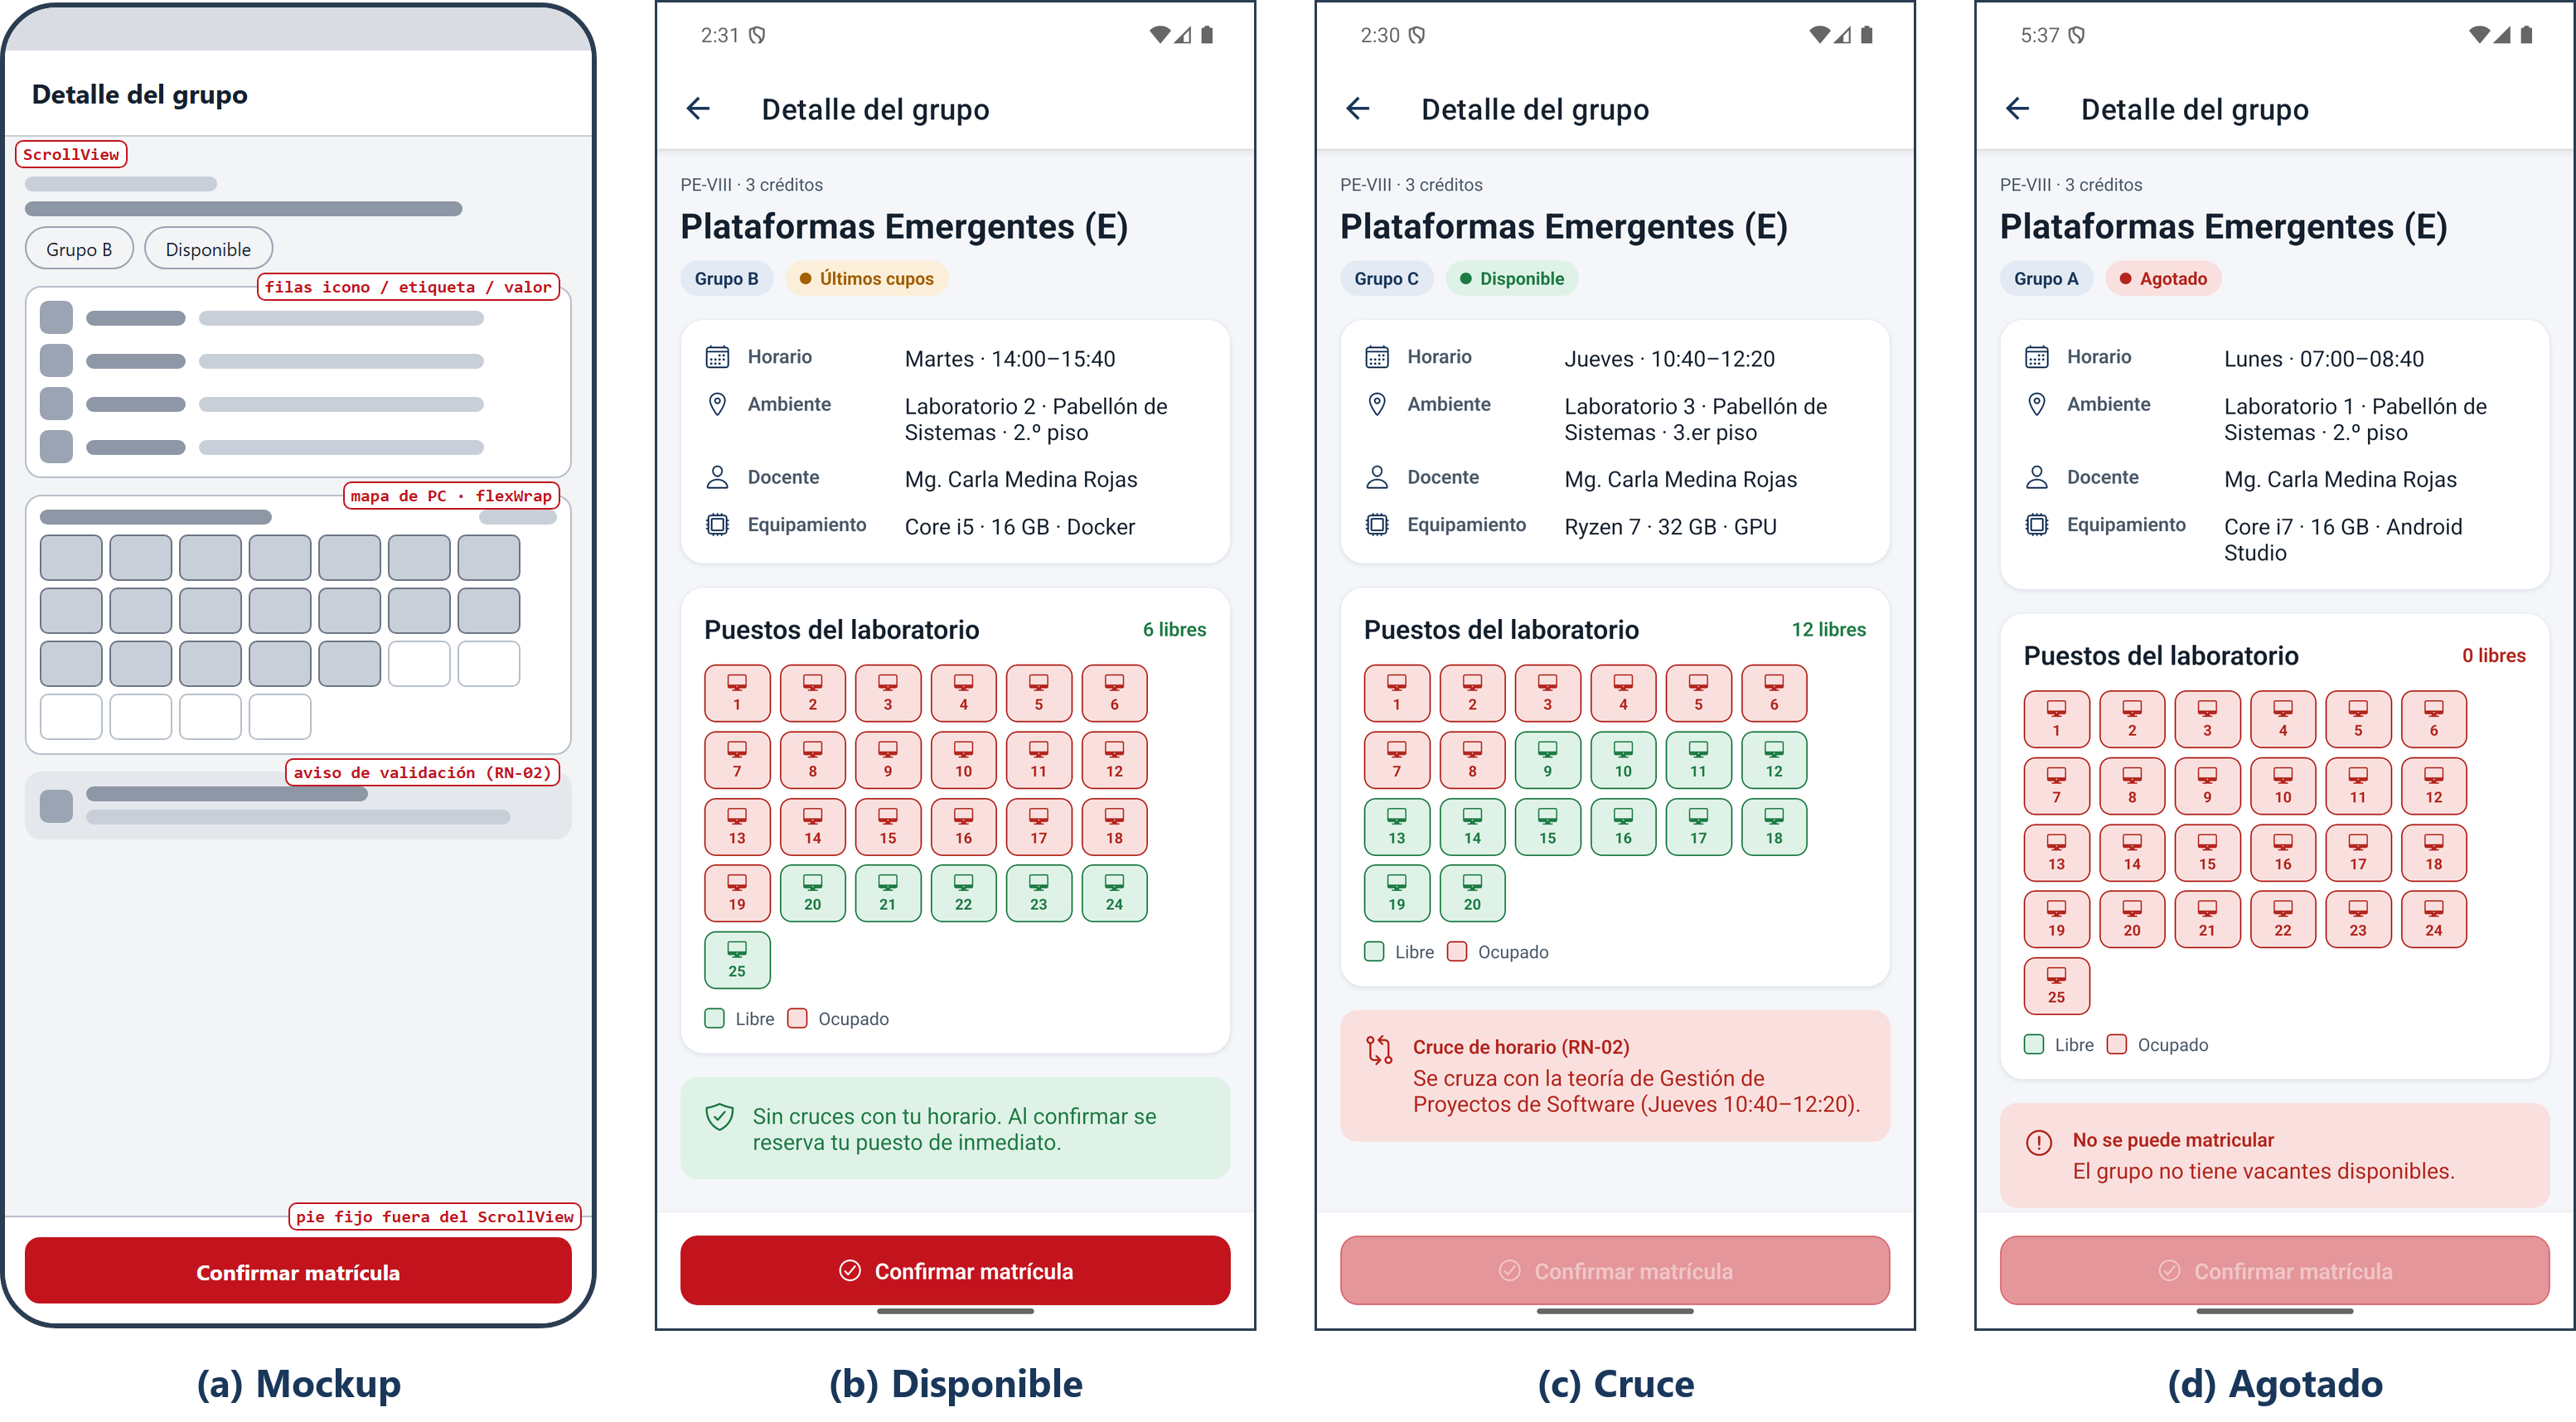
\includegraphics[width=0.78\textwidth]{img/figuras/fig_i04.png}\\[0.2cm]
{\small\itshape MatriLab EPIS ejecutándose en Android: mockup, grupo disponible, bloqueo por cruce de horario y grupo agotado.}
\end{center}
\clearpage

\renewcommand{\contentsname}{\textcolor{colabpyblue}{Índice General de Contenidos}}
{
  \hypersetup{linkcolor=colabpyblue}
  \setcounter{tocdepth}{2}
  \small
  \tableofcontents
}
\clearpage
{\hypersetup{linkcolor=colabpyblue}\listoffigures}
\vspace{0.6cm}
{\hypersetup{linkcolor=colabpyblue}\listoftables}
\clearpage
\seccionInforme{1. Descripción general del programa}
\phantomsection\addcontentsline{toc}{section}{1. Descripción general del programa}

\vspace{0.2cm}
\phantomsection\addcontentsline{toc}{subsection}{1.1 Contexto y propósito}
\colabtitle{1.1 Contexto y propósito}

\textbf{MatriLab EPIS} es una aplicación móvil para gestionar la matrícula en los grupos de laboratorio de la Escuela Profesional de Ingeniería de Sistemas de la UNSA. Es el mismo dominio que el equipo trabajó en el LAB 01 (selección de herramienta y requisitos) y en el LAB 02 (prototipo RMAD en FlutterFlow). En esta práctica la aplicación se reconstruye con un \textbf{framework multiplataforma}, \textbf{React Native}, usando únicamente los componentes propios de la plataforma para organizar cada interfaz.

El programa atiende a tres usuarios. El \textbf{estudiante} consulta la oferta de grupos con un semáforo de vacantes, se matricula sin cruces de horario y obtiene un pase digital con código QR. El \textbf{docente o jefe de prácticas} revisa la nómina de sus grupos y registra la asistencia leyendo el QR con la cámara del teléfono. La \textbf{coordinación de laboratorios} define la capacidad de cada ambiente y la ventana de matrícula. Las doce pantallas comparten un mismo código que se ejecuta como aplicación nativa en Android y como aplicación web.

Los datos de esta versión son de demostración y viven en memoria: el objetivo de la práctica es el diseño y la organización de las interfaces. Las reglas de negocio (cruce de horarios, aforo, ventana de matrícula y verificación del pase) sí son reales y se verifican con pruebas automatizadas.

\vspace{0.2cm}
\phantomsection\addcontentsline{toc}{subsection}{1.2 Árbol de problemas}
\colabtitle{1.2 Árbol de problemas}

El diseño parte del diagnóstico del LAB 01 sobre el proceso de matrícula de laboratorios. Se aplicó la técnica del árbol de problemas de la metodología del marco lógico [17]: un problema central, sus causas directas e indirectas y los efectos que produce (Figura \ref{fig:arbol_problemas}).

\begin{figure}[!htbp]
\centering
\safeimage{1.0\textwidth}{img/diagramas/arbol_problemas.png}{Árbol de problemas del proceso de matrícula de laboratorios de la EPIS-UNSA}
\caption{Árbol de problemas del proceso de matrícula de laboratorios de la EPIS-UNSA}
\label{fig:arbol_problemas}
\end{figure}

El problema central es que \textbf{la matrícula en los laboratorios es lenta, poco transparente y genera sobrecupos y cruces de horario}. Las causas de fondo son listas que no se actualizan en tiempo real, la falta de contraste entre el grupo práctico y la teoría inscrita, inscripciones simultáneas sin una operación atómica, la ausencia de una constancia digital y la coordinación de las salas por correo. Los efectos llegan al aula: rechazos al final del trámite, permutas cuando las clases ya empezaron, salas con más estudiantes que computadoras y nóminas tardías.

\vspace{0.2cm}
\phantomsection\addcontentsline{toc}{subsection}{1.3 Árbol de objetivos y alcance}
\colabtitle{1.3 Árbol de objetivos y alcance}

Cada condición negativa se convirtió en la situación deseada (Figura \ref{fig:arbol_objetivos}). Los \textbf{medios fundamentales}, en la base del árbol, son acciones concretas que el software puede ejecutar; por eso se tomaron como origen de las funcionalidades. Debajo de cada medio se indican las interfaces de MatriLab que lo implementan.

\begin{figure}[!htbp]
\centering
\safeimage{1.0\textwidth}{img/diagramas/arbol_objetivos.png}{Árbol de objetivos: los medios fundamentales se traducen en interfaces de MatriLab}
\caption{Árbol de objetivos: los medios fundamentales se traducen en interfaces de MatriLab}
\label{fig:arbol_objetivos}
\end{figure}

El alcance de la práctica cubre los cinco medios con \textbf{doce interfaces} (I1 a I12). La autenticación real con Google Workspace y la persistencia en la nube, que en el LAB 02 se resolvieron con Firebase, se simulan aquí con un inicio de sesión de demostración y un estado local, de modo que cualquier evaluador puede probar la aplicación sin cuentas ni conexión.

\vspace{0.2cm}
\phantomsection\addcontentsline{toc}{subsection}{1.4 Actores y requisitos atendidos}
\colabtitle{1.4 Actores y requisitos atendidos}

\begin{table}[H]
\centering\small
\caption{Actores del sistema y lo que cada uno puede hacer en la aplicación}\label{tab:actores}
\renewcommand{\arraystretch}{1.25}
\begin{tabular}{|>{\raggedright\arraybackslash}p{\dimexpr 0.170\linewidth-2\tabcolsep-2\arrayrulewidth\relax}|>{\raggedright\arraybackslash}p{\dimexpr 0.220\linewidth-2\tabcolsep-2\arrayrulewidth\relax}|>{\raggedright\arraybackslash}p{\dimexpr 0.460\linewidth-2\tabcolsep-2\arrayrulewidth\relax}|>{\raggedright\arraybackslash}p{\dimexpr 0.150\linewidth-2\tabcolsep-2\arrayrulewidth\relax}|}
\hline
\rowcolor{colabpyblue} \color{white}\textbf{Rol} & \color{white}\textbf{Cuenta de demostración} & \color{white}\textbf{Responsabilidades en MatriLab} & \color{white}\textbf{Interfaces} \\ \hline
Estudiante & Lopez Arela, Ower Frank · CUI 20213412 & Consultar la oferta, matricularse sin cruces, ver su horario, mostrar su pase QR y anular una matrícula dentro de la ventana. & I1–I6, I12 \\ \hline
\rowcolor{colabpybg} Docente / jefe de prácticas & Mg. Carla Medina Rojas (ficticia) & Revisar la ocupación de sus grupos, consultar la nómina, registrar asistencia con QR o código manual y exportar la nómina. & I1, I7–I9, I12 \\ \hline
Coordinación de laboratorios & \texttt{laboratorios.\allowbreak{}epis@unsa.\allowbreak{}edu.\allowbreak{}pe} & Ajustar capacidad y estado de cada ambiente, definir la ventana de matrícula y revisar los grupos agotados. & I1, I10–I12 \\ \hline
\end{tabular}
\end{table}

\begin{table}[H]
\centering\small
\caption{Requisitos funcionales del LAB 01 y cómo se resuelven en la aplicación}\label{tab:rf}
\renewcommand{\arraystretch}{1.25}
\begin{tabular}{|>{\raggedright\arraybackslash}p{\dimexpr 0.090\linewidth-2\tabcolsep-2\arrayrulewidth\relax}|>{\raggedright\arraybackslash}p{\dimexpr 0.250\linewidth-2\tabcolsep-2\arrayrulewidth\relax}|>{\raggedright\arraybackslash}p{\dimexpr 0.510\linewidth-2\tabcolsep-2\arrayrulewidth\relax}|>{\raggedright\arraybackslash}p{\dimexpr 0.150\linewidth-2\tabcolsep-2\arrayrulewidth\relax}|}
\hline
\rowcolor{colabpyblue} \color{white}\textbf{Código} & \color{white}\textbf{Requisito} & \color{white}\textbf{Cómo se resuelve} & \color{white}\textbf{Interfaz} \\ \hline
RF-01 & Autenticación institucional & Validación del dominio @unsa.edu.pe y de la contraseña; acceso de demostración por rol. & I1 \\ \hline
\rowcolor{colabpybg} RF-02 & Catálogo de cursos y grupos & Lista agrupada por curso con buscador y filtros. & I3 \\ \hline
RF-03 & Vacantes en vivo & Semáforo y barra de ocupación que se recalculan al matricular o anular. & I2, I3, I4 \\ \hline
\rowcolor{colabpybg} RF-04 & Validación anti-cruces & Contraste del grupo con los laboratorios y la teoría inscritos (RN-02). & I4 \\ \hline
RF-05 & Reserva atómica & El cupo se descuenta y la matrícula se registra en una sola operación. & I4 \\ \hline
\rowcolor{colabpybg} RF-06 & Ficha digital con QR & Pase con código QR firmado y código de verificación de 8 caracteres. & I5 \\ \hline
RF-07 & Horario consolidado y nómina & Cuadrícula semanal con teoría y laboratorios; nómina por grupo. & I6, I7, I8 \\ \hline
\rowcolor{colabpybg} RF-08 & Asistencia por escaneo QR & Cámara del teléfono con lector QR o ingreso manual del código. & I9 \\ \hline
RF-09 & Parametrización de laboratorios & Capacidad, estado y datos de cada sala; ventana de matrícula validada. & I10, I11 \\ \hline
\rowcolor{colabpybg} RF-10 & Exportación de nóminas & CSV con separador punto y coma compartido con la hoja nativa del sistema. & I8 \\ \hline
\end{tabular}
\end{table}

\vspace{0.2cm}
\phantomsection\addcontentsline{toc}{subsection}{1.5 Elección del framework}
\colabtitle{1.5 Elección del framework}

La guía permite Flutter, React Native o Xamarin. El equipo eligió \textbf{React Native 0.88 con Expo SDK 58} por tres razones. Primero, React Native dibuja la interfaz con \textbf{vistas nativas} de cada sistema operativo: un \texttt{View} es un \texttt{View\allowbreak{}Group} en Android y un \texttt{UIView} en iOS [2], lo que responde directamente al requisito de usar los componentes propios de la plataforma. Segundo, el LAB 02 ya se había construido sobre Flutter mediante FlutterFlow, y usar otro framework permite comparar ambos enfoques con evidencia propia. Tercero, Expo [14] permite ejecutar la aplicación en un emulador o teléfono con Expo Go sin compilar proyectos nativos y exportarla a la web con el mismo código. Se complementó con TypeScript, React Navigation 7 para la navegación nativa, \texttt{expo-camera} para el lector QR y Jest para las pruebas.


\clearpage
\seccionInforme{2. Diseño de interfaces}
\phantomsection\addcontentsline{toc}{section}{2. Diseño de interfaces}

\vspace{0.2cm}
\phantomsection\addcontentsline{toc}{subsection}{2.1 Funcionalidades derivadas del árbol de objetivos}
\colabtitle{2.1 Funcionalidades derivadas del árbol de objetivos}

Cada medio fundamental del árbol de objetivos se descompuso en funcionalidades concretas. La Tabla 4 muestra esa trazabilidad, que es la base del diseño: ninguna pantalla se agregó sin un medio que la justifique.

\begin{table}[H]
\centering\small
\caption{Trazabilidad entre medios del árbol de objetivos, funcionalidades e interfaces}
\renewcommand{\arraystretch}{1.25}
\begin{tabular}{|>{\raggedright\arraybackslash}p{\dimexpr 0.240\linewidth-2\tabcolsep-2\arrayrulewidth\relax}|>{\raggedright\arraybackslash}p{\dimexpr 0.530\linewidth-2\tabcolsep-2\arrayrulewidth\relax}|>{\raggedright\arraybackslash}p{\dimexpr 0.230\linewidth-2\tabcolsep-2\arrayrulewidth\relax}|}
\hline
\rowcolor{colabpyblue} \color{white}\textbf{Medio} & \color{white}\textbf{Funcionalidad} & \color{white}\textbf{Interfaz} \\ \hline
1.1 Catálogo conectado & F-01 Iniciar sesión con correo institucional y elegir rol & I1 Inicio de sesión \\ \hline
\rowcolor{colabpybg} 1.1 Catálogo conectado & F-02 Ver resumen personal: ventana, créditos, vacantes y laboratorios matriculados & I2 Panel del estudiante \\ \hline
1.1 Catálogo conectado & F-03 Explorar grupos por curso con semáforo, buscador y filtros & I3 Catálogo \\ \hline
\rowcolor{colabpybg} 2.1 Contraste de horario & F-04 Revisar el detalle del grupo y el mapa de puestos; validar cruces antes de confirmar & I4 Detalle del grupo \\ \hline
2.1 Contraste de horario & F-05 Consultar el horario semanal con teoría y laboratorios & I6 Horario \\ \hline
\rowcolor{colabpybg} 3.1 Operación única & F-06 Confirmar la matrícula con reserva atómica del cupo & I4 Detalle del grupo \\ \hline
4.1 Código verificable & F-07 Mostrar y compartir el pase con QR y código de verificación & I5 Pase QR \\ \hline
\rowcolor{colabpybg} 4.1 Código verificable & F-08 Monitorear la ocupación de los grupos del docente & I7 Panel docente \\ \hline
4.1 Código verificable & F-09 Consultar la nómina, marcar asistencia y exportar CSV & I8 Nómina \\ \hline
\rowcolor{colabpybg} 4.1 Código verificable & F-10 Leer el QR con la cámara o digitar el código & I9 Escáner \\ \hline
5.1 Parametrización & F-11 Ajustar capacidad, estado y datos de cada laboratorio & I10 Laboratorios \\ \hline
\rowcolor{colabpybg} 5.1 Parametrización & F-12 Configurar la ventana de matrícula y las reglas; revisar grupos agotados & I11 Matrícula \\ \hline
Transversal & F-13 Elegir tema claro u oscuro, ajustar avisos y cerrar sesión & I12 Perfil \\ \hline
\end{tabular}
\end{table}

\vspace{0.2cm}
\phantomsection\addcontentsline{toc}{subsection}{2.2 Mapa de navegación}
\colabtitle{2.2 Mapa de navegación}

La estructura de navegación se definió antes de dibujar las pantallas (Figura 3). Una \textbf{pila nativa} raíz contiene el inicio de sesión, tres navegadores de \textbf{pestañas inferiores} (uno por rol) y tres pantallas que se apilan sobre las pestañas: el detalle del grupo, que se presenta como hoja modal, el pase QR y la nómina. Así cada rol ve solo sus opciones y el botón Atrás del sistema se comporta como el usuario espera.

\begin{figure}[H]
\centering
\safeimage{1.0\textwidth}{img/diagramas/navegacion.png}{Mapa de navegación de MatriLab: pila nativa raíz y pestañas por rol}
\caption{Mapa de navegación de MatriLab: pila nativa raíz y pestañas por rol}
\label{fig:navegacion}
\end{figure}

\vspace{0.2cm}
\phantomsection\addcontentsline{toc}{subsection}{2.3 Sistema visual}
\colabtitle{2.3 Sistema visual}

Para que las doce interfaces se vean consistentes se definieron \textit{tokens} de diseño en \texttt{src/\allowbreak{}theme/\allowbreak{}tokens.\allowbreak{}ts}. Se conservaron los colores institucionales usados desde el LAB 01 y se definió una variante oscura de cada color, ya que la aplicación sigue el tema del sistema operativo.

\begin{table}[H]
\centering\small
\caption{Tokens de diseño de la aplicación}
\renewcommand{\arraystretch}{1.25}
\begin{tabular}{|>{\raggedright\arraybackslash}p{\dimexpr 0.200\linewidth-2\tabcolsep-2\arrayrulewidth\relax}|>{\raggedright\arraybackslash}p{\dimexpr 0.270\linewidth-2\tabcolsep-2\arrayrulewidth\relax}|>{\raggedright\arraybackslash}p{\dimexpr 0.200\linewidth-2\tabcolsep-2\arrayrulewidth\relax}|>{\raggedright\arraybackslash}p{\dimexpr 0.330\linewidth-2\tabcolsep-2\arrayrulewidth\relax}|}
\hline
\rowcolor{colabpyblue} \color{white}\textbf{Token} & \color{white}\textbf{Claro} & \color{white}\textbf{Oscuro} & \color{white}\textbf{Uso} \\ \hline
primario & \#19375A & \#7FA7D9 & Botones principales, cabeceras de tarjetas, grupo seleccionado. \\ \hline
\rowcolor{colabpybg} marca & \#C3141E & \#FF6B6B & Acciones decisivas (Ingresar, Confirmar matrícula) y pestaña activa. \\ \hline
éxito / alerta / peligro & \#1E7B45 / \#A35F00 / \#B3261E & variantes claras & Semáforo de vacantes: verde, ámbar y rojo. \\ \hline
\rowcolor{colabpybg} fondo / superficie & \#F4F6F9 / \#FFFFFF & \#0F1720 / \#17212C & Fondo de pantalla y de tarjetas. \\ \hline
espacio & 4 · 8 · 12 · 16 · 24 · 32 & igual & Escala de 4 pt para márgenes, rellenos y \texttt{gap}. \\ \hline
\rowcolor{colabpybg} radio & 8 · 12 · 16 · 999 & igual & Esquinas de controles, tarjetas y píldoras. \\ \hline
tipo & 26 · 18 · 15 · 13 · 12 & igual & Título, subtítulo, cuerpo, etiqueta y pie (en dp). \\ \hline
\end{tabular}
\end{table}

\vspace{0.2cm}
\phantomsection\addcontentsline{toc}{subsection}{2.4 Mockups de baja fidelidad}
\colabtitle{2.4 Mockups de baja fidelidad}

Con las funcionalidades y la navegación definidas se dibujaron mockups de baja fidelidad para las doce interfaces (Figuras 4 y 5). Se usaron solo grises, sin textos reales, para discutir la \textbf{organización} de cada pantalla antes que su apariencia. Cada región lleva una etiqueta roja con el componente de React Native previsto y los recuadros discontinuos marcan contenedores de layout (filas, columnas o listas). Ese mismo boceto guió luego la implementación: en la sección 4.6 cada mockup aparece junto a la captura real de la pantalla.

\begin{figure}[H]
\centering
\safeimage{0.8\textwidth}{img/diagramas/mockups_estudiante.png}{Mockups de baja fidelidad de las interfaces del estudiante (I1 a I6)}
\caption{Mockups de baja fidelidad de las interfaces del estudiante (I1 a I6)}
\label{fig:mockups_e}
\end{figure}

\begin{figure}[H]
\centering
\safeimage{0.8\textwidth}{img/diagramas/mockups_docente_admin.png}{Mockups de baja fidelidad de las interfaces del docente y de administración (I7 a I12)}
\caption{Mockups de baja fidelidad de las interfaces del docente y de administración (I7 a I12)}
\label{fig:mockups_d}
\end{figure}

Las decisiones de organización más importantes que quedaron fijadas en los mockups fueron las siguientes:

\begin{itemize}[label=\textcolor{unsared}{\textbullet}, leftmargin=*]
    \item \textbf{Listas largas virtualizadas.} El catálogo, el panel docente, la nómina y los laboratorios se planificaron como \texttt{Section\allowbreak{}List} o \texttt{Flat\allowbreak{}List}, nunca como un \texttt{Scroll\allowbreak{}View} con muchos hijos.
    \item \textbf{Acción principal fija.} En el detalle del grupo y en la nómina el botón principal queda en un pie fuera del área desplazable, siempre visible.
    \item \textbf{Superposiciones con posición absoluta.} El sello del pase, la guía de encuadre del escáner y los bloques del horario se colocan con \texttt{position: 'absolute'} sobre su contenedor.
    \item \textbf{Cuadrículas que se reacomodan.} Los indicadores (KPI) y el mapa de puestos usan \texttt{flex\allowbreak{}Wrap}, de modo que el número de columnas depende del ancho disponible y no de valores fijos.
\end{itemize}

\vspace{0.2cm}
\phantomsection\addcontentsline{toc}{subsection}{2.5 Criterios de usabilidad y accesibilidad}
\colabtitle{2.5 Criterios de usabilidad y accesibilidad}

\begin{itemize}[label=\textcolor{unsared}{\textbullet}, leftmargin=*]
    \item Área táctil mínima de \textbf{48 dp} en botones y campos (\texttt{min\allowbreak{}Height: 48}), y \texttt{hit\allowbreak{}Slop} en iconos pequeños.
    \item Todos los controles tienen \texttt{accessibility\allowbreak{}Label} y \texttt{accessibility\allowbreak{}Role}; las filas de la nómina se anuncian como casillas (\texttt{accessibility\allowbreak{}Role=\allowbreak{}"checkbox"}) con su estado.
    \item Los mensajes de error y de validación usan \texttt{accessibility\allowbreak{}Live\allowbreak{}Region} para que el lector de pantalla los lea al aparecer.
    \item El semáforo nunca depende solo del color: siempre va acompañado del texto \textit{Disponible}, \textit{Últimos cupos} o \textit{Agotado}.
    \item Tema claro y oscuro con contraste suficiente; la escala de texto del sistema (\texttt{font\allowbreak{}Scale}) se respeta y se muestra en el perfil.
\end{itemize}


\clearpage
\seccionInforme{3. Componentes de React Native para la organización de la interfaz}
\phantomsection\addcontentsline{toc}{section}{3. Componentes de React Native para la organización de la interfaz}

\vspace{0.2cm}
\phantomsection\addcontentsline{toc}{subsection}{3.1 Cómo dibuja React Native una interfaz}
\colabtitle{3.1 Cómo dibuja React Native una interfaz}

En React Native la interfaz se describe con componentes de React escritos en JavaScript o TypeScript, pero lo que aparece en pantalla no es HTML: el renderizador \textbf{Fabric} traduce cada componente del núcleo a una vista nativa del sistema operativo [2], [13]. Las posiciones y tamaños se calculan con \textbf{Yoga}, un motor de layout multiplataforma que implementa el modelo Flexbox [15]. La Tabla 6 resume la correspondencia documentada para los componentes básicos.

\begin{table}[H]
\centering\small
\caption{Componentes del núcleo y la vista nativa que los representa en cada plataforma (según [2])}
\renewcommand{\arraystretch}{1.25}
\begin{tabular}{|>{\raggedright\arraybackslash}p{\dimexpr 0.150\linewidth-2\tabcolsep-2\arrayrulewidth\relax}|>{\raggedright\arraybackslash}p{\dimexpr 0.150\linewidth-2\tabcolsep-2\arrayrulewidth\relax}|>{\raggedright\arraybackslash}p{\dimexpr 0.150\linewidth-2\tabcolsep-2\arrayrulewidth\relax}|>{\raggedright\arraybackslash}p{\dimexpr 0.190\linewidth-2\tabcolsep-2\arrayrulewidth\relax}|>{\raggedright\arraybackslash}p{\dimexpr 0.360\linewidth-2\tabcolsep-2\arrayrulewidth\relax}|}
\hline
\rowcolor{colabpyblue} \color{white}\textbf{Componente} & \color{white}\textbf{Android} & \color{white}\textbf{iOS} & \color{white}\textbf{Web (react-native-web)} & \color{white}\textbf{Función} \\ \hline
\texttt{<View>} & ViewGroup & UIView & \texttt{<div>} & Contenedor con flexbox, estilo, toques y accesibilidad. \\ \hline
\rowcolor{colabpybg} \texttt{<Text>} & TextView & UITextView & \texttt{<p>} & Muestra y anida texto con estilos. \\ \hline
\texttt{<Image>} & ImageView & UIImageView & \texttt{<img>} & Muestra imágenes locales o remotas. \\ \hline
\rowcolor{colabpybg} \texttt{<Scroll\allowbreak{}View>} & ScrollView & UIScrollView & \texttt{<div>} desplazable & Contenedor genérico con desplazamiento. \\ \hline
\texttt{<Text\allowbreak{}Input>} & EditText & UITextField & \texttt{<input>} & Entrada de texto con teclado del sistema. \\ \hline
\end{tabular}
\end{table}

Esta correspondencia explica por qué una aplicación React Native se siente propia de cada sistema: el \texttt{Switch} de la configuración es el interruptor de Android, el teclado es el del teléfono y la pila de navegación usa las transiciones nativas. A la vez, todo se describe con un solo árbol de componentes, que es lo que permite compartir el código.

\vspace{0.2cm}
\phantomsection\addcontentsline{toc}{subsection}{3.2 Flexbox en React Native}
\colabtitle{3.2 Flexbox en React Native}

Toda la organización espacial se hace con Flexbox. Un contenedor define un \textbf{eje principal} (\texttt{flex\allowbreak{}Direction}) y distribuye a sus hijos a lo largo de él (\texttt{justify\allowbreak{}Content}) y del eje transversal (\texttt{align\allowbreak{}Items}). La documentación oficial advierte que, aunque el modelo es el de CSS, \textbf{los valores por defecto cambian} [1]:

\begin{itemize}[label=\textcolor{unsared}{\textbullet}, leftmargin=*]
    \item \texttt{flex\allowbreak{}Direction} vale \texttt{'column'} (en la web vale \texttt{'row'}): por eso, sin indicar nada, los hijos se apilan.
    \item \texttt{align\allowbreak{}Content} vale \texttt{'flex-start'} en lugar de \texttt{'stretch'}.
    \item \texttt{flex\allowbreak{}Shrink} vale \texttt{0} en lugar de \texttt{1}: un hijo no se encoge salvo que se indique.
    \item \texttt{flex} acepta un solo número, no la forma abreviada de tres valores de CSS.
\end{itemize}

La Figura 6 reproduce, con las mismas propiedades que usa la app, los ocho patrones de layout que más se repiten en MatriLab.

\begin{figure}[H]
\centering
\safeimage{1.0\textwidth}{img/diagramas/flexbox.png}{Patrones de layout con Flexbox utilizados en MatriLab}
\caption{Patrones de layout con Flexbox utilizados en MatriLab}
\label{fig:flexbox}
\end{figure}

\begin{table}[H]
\centering\small
\caption{Propiedades de layout más usadas y dónde se aplican}
\renewcommand{\arraystretch}{1.25}
\begin{tabular}{|>{\raggedright\arraybackslash}p{\dimexpr 0.240\linewidth-2\tabcolsep-2\arrayrulewidth\relax}|>{\raggedright\arraybackslash}p{\dimexpr 0.300\linewidth-2\tabcolsep-2\arrayrulewidth\relax}|>{\raggedright\arraybackslash}p{\dimexpr 0.460\linewidth-2\tabcolsep-2\arrayrulewidth\relax}|}
\hline
\rowcolor{colabpyblue} \color{white}\textbf{Propiedad} & \color{white}\textbf{Valores usados} & \color{white}\textbf{Ejemplo en MatriLab} \\ \hline
\texttt{flex\allowbreak{}Direction} & \texttt{'row'}, \texttt{'column'} & Filas icono/texto/acción; formularios en columna. \\ \hline
\rowcolor{colabpybg} \texttt{flex} & \texttt{1} & El texto de una fila ocupa el espacio que dejan avatar e insignia. \\ \hline
\texttt{justify\allowbreak{}Content} & \texttt{'space-between'}, \texttt{'center'} & Cabecera de tarjeta con título e insignia; botones centrados. \\ \hline
\rowcolor{colabpybg} \texttt{align\allowbreak{}Items} / \texttt{align\allowbreak{}Self} & \texttt{'center'}, \texttt{'flex-start'}, \texttt{'stretch'} & Insignias que no se estiran; columna de datos del pase. \\ \hline
\texttt{flex\allowbreak{}Wrap} + \texttt{gap} & \texttt{'wrap'}, 6–12 dp & Mapa de puestos del laboratorio y KPI en dos columnas. \\ \hline
\rowcolor{colabpybg} \texttt{flex\allowbreak{}Basis} / \texttt{flex\allowbreak{}Grow} & \texttt{'47\%'}, \texttt{1} & Cada KPI ocupa media fila y absorbe el sobrante. \\ \hline
\texttt{position} & \texttt{'absolute'} con \texttt{top/\allowbreak{}left/\allowbreak{}right/\allowbreak{}bottom} & Sello del pase, guía del escáner, bloques del horario. \\ \hline
\rowcolor{colabpybg} \texttt{width} en porcentaje & \texttt{'50\%'} y porcentajes calculados & Datos del pase en dos columnas; relleno de la barra de ocupación. \\ \hline
\end{tabular}
\end{table}

\vspace{0.2cm}
\phantomsection\addcontentsline{toc}{subsection}{3.3 Contenedores de organización}
\colabtitle{3.3 Contenedores de organización}

\begin{itemize}[label=\textcolor{unsared}{\textbullet}, leftmargin=*]
    \item \textbf{View.} Es el bloque de construcción de toda pantalla. En MatriLab no se usa ninguna librería de componentes visuales: tarjetas, botones, chips, insignias y barras de progreso se construyeron sobre \texttt{View}, \texttt{Text} y \texttt{Pressable} (archivo \texttt{src/\allowbreak{}components/\allowbreak{}ui.\allowbreak{}tsx}).
    \item \textbf{SafeAreaView.} Evita que el contenido quede bajo la barra de estado o la muesca. La documentación de React Native marca el \texttt{Safe\allowbreak{}Area\allowbreak{}View} del núcleo como obsoleto y recomienda \texttt{react-native-safe-area-context} [16], que funciona también en Android; la aplicación usa este último en el inicio de sesión y con \texttt{Safe\allowbreak{}Area\allowbreak{}Provider} en la raíz.
    \item \textbf{ScrollView.} Contenedor desplazable que monta todos sus hijos a la vez [3]. Se reserva para pantallas de contenido acotado: panel del estudiante, detalle del grupo, pase QR, horario, configuración y perfil. Con \texttt{horizontal} se usa para la fila de filtros del catálogo y para el horario cuando la pantalla es angosta.
    \item \textbf{KeyboardAvoidingView.} Ajusta el espacio cuando aparece el teclado [8]. Su comportamiento difiere por plataforma, por eso se usa \texttt{behavior=\allowbreak{}\{Platform.\allowbreak{}OS =\allowbreak{}=\allowbreak{}=\allowbreak{} 'ios' ? 'padding' : 'height'\}} en el inicio de sesión y en el escáner.
    \item \textbf{Modal.} Presenta contenido sobre la pantalla actual [9]. Con \texttt{transparent} y \texttt{animation\allowbreak{}Type=\allowbreak{}"slide"} se construyó una hoja inferior para editar los datos de un laboratorio; \texttt{on\allowbreak{}Request\allowbreak{}Close} atiende el botón Atrás de Android.
\end{itemize}

\vspace{0.2cm}
\phantomsection\addcontentsline{toc}{subsection}{3.4 Listas virtualizadas}
\colabtitle{3.4 Listas virtualizadas}

Cuando la cantidad de elementos crece, un \texttt{Scroll\allowbreak{}View} desperdicia memoria porque dibuja todo aunque no se vea. \texttt{Flat\allowbreak{}List} y \texttt{Section\allowbreak{}List} solo montan los elementos cercanos a la zona visible y reciclan el resto [4], [5], [18]. La Tabla 8 resume cómo se configuró cada lista.

\begin{table}[H]
\centering\small
\caption{Configuración de las listas virtualizadas de la aplicación}
\renewcommand{\arraystretch}{1.25}
\begin{tabular}{|>{\raggedright\arraybackslash}p{\dimexpr 0.150\linewidth-2\tabcolsep-2\arrayrulewidth\relax}|>{\raggedright\arraybackslash}p{\dimexpr 0.140\linewidth-2\tabcolsep-2\arrayrulewidth\relax}|>{\raggedright\arraybackslash}p{\dimexpr 0.380\linewidth-2\tabcolsep-2\arrayrulewidth\relax}|>{\raggedright\arraybackslash}p{\dimexpr 0.330\linewidth-2\tabcolsep-2\arrayrulewidth\relax}|}
\hline
\rowcolor{colabpyblue} \color{white}\textbf{Interfaz} & \color{white}\textbf{Componente} & \color{white}\textbf{Propiedades clave} & \color{white}\textbf{Motivo} \\ \hline
I3 Catálogo & \texttt{Section\allowbreak{}List} & \texttt{sections}, \texttt{render\allowbreak{}Section\allowbreak{}Header}, \texttt{sticky\allowbreak{}Section\allowbreak{}Headers\allowbreak{}Enabled}, \texttt{List\allowbreak{}Empty\allowbreak{}Component} & Agrupar los grupos por curso con el nombre del curso fijo arriba al desplazarse. \\ \hline
\rowcolor{colabpybg} I7 Panel docente & \texttt{Flat\allowbreak{}List} & \texttt{List\allowbreak{}Header\allowbreak{}Component}, \texttt{Item\allowbreak{}Separator\allowbreak{}Component} & Saludo y KPI dentro de la misma lista, sin anidar listas en un \texttt{Scroll\allowbreak{}View}. \\ \hline
I8 Nómina & \texttt{Flat\allowbreak{}List} & \texttt{sticky\allowbreak{}Header\allowbreak{}Indices=\allowbreak{}\{[0]\}}, filas de alto fijo & Resumen de asistencia y buscador siempre visibles sobre la lista de estudiantes. \\ \hline
\rowcolor{colabpybg} I10 Laboratorios & \texttt{Flat\allowbreak{}List} & \texttt{num\allowbreak{}Columns}, \texttt{column\allowbreak{}Wrapper\allowbreak{}Style}, \texttt{key=\allowbreak{}\{columnas\}} & Rejilla de 1, 2 o 3 columnas según el ancho de la ventana. \\ \hline
\end{tabular}
\end{table}

\begin{notaInfo}
\texttt{num\allowbreak{}Columns} no puede cambiar mientras la lista está montada. Por eso en I10 la propiedad \texttt{key} depende del número de columnas: al girar el teléfono React desmonta la lista y la vuelve a crear con la nueva rejilla.
\end{notaInfo}

\vspace{0.2cm}
\phantomsection\addcontentsline{toc}{subsection}{3.5 Posicionamiento, dimensiones y adaptación}
\colabtitle{3.5 Posicionamiento, dimensiones y adaptación}

\begin{itemize}[label=\textcolor{unsared}{\textbullet}, leftmargin=*]
    \item \textbf{\texttt{position: 'absolute'}} saca a un elemento del flujo y lo ubica respecto de su contenedor. \texttt{Style\allowbreak{}Sheet.\allowbreak{}absolute\allowbreak{}Fill} es el atajo para cubrirlo por completo, como hace la vista de cámara del escáner.
    \item \textbf{Porcentajes.} \texttt{width} y \texttt{height} aceptan porcentajes del contenedor [12]; el relleno de la barra de ocupación recibe como ancho el porcentaje calculado de puestos ocupados.
    \item \textbf{useWindowDimensions} devuelve el ancho y alto de la ventana y se actualiza solo al rotar o redimensionar [10]. Con él se calculan el ancho de cada día del horario, el tamaño del QR y las columnas de la lista de laboratorios.
    \item \textbf{Platform} permite pequeñas diferencias por sistema (\texttt{Platform.\allowbreak{}OS}, \texttt{Platform.\allowbreak{}Version}) [11].
    \item \textbf{StyleSheet} agrupa los estilos de cada archivo y ofrece \texttt{hairline\allowbreak{}Width}, la línea más fina que puede dibujar la pantalla, usada en bordes y separadores [6].
    \item \textbf{useColorScheme} informa si el sistema está en modo claro u oscuro; el \texttt{Theme\allowbreak{}Context} lo usa para elegir la paleta.
\end{itemize}

\vspace{0.2cm}
\phantomsection\addcontentsline{toc}{subsection}{3.6 Componentes de interacción y retroalimentación}
\colabtitle{3.6 Componentes de interacción y retroalimentación}

\begin{table}[H]
\centering\small
\caption{Componentes de interacción utilizados}
\renewcommand{\arraystretch}{1.25}
\begin{tabular}{|>{\raggedright\arraybackslash}p{\dimexpr 0.280\linewidth-2\tabcolsep-2\arrayrulewidth\relax}|>{\raggedright\arraybackslash}p{\dimexpr 0.720\linewidth-2\tabcolsep-2\arrayrulewidth\relax}|}
\hline
\rowcolor{colabpyblue} \color{white}\textbf{Componente o API} & \color{white}\textbf{Uso en MatriLab} \\ \hline
\texttt{Pressable} & Base de botones, chips, tarjetas tocables y filas de la nómina. Su \texttt{style} recibe \texttt{pressed} para el efecto visual y en Android se agrega \texttt{android\_\allowbreak{}ripple} [7]. \\ \hline
\rowcolor{colabpybg} \texttt{Text\allowbreak{}Input} & Correo y contraseña (\texttt{secure\allowbreak{}Text\allowbreak{}Entry}), buscadores, fechas de la ventana y código de verificación filtrado a hexadecimal. \\ \hline
\texttt{Switch} & Mantener sesión, habilitar laboratorio, reglas de matrícula y avisos del perfil. \\ \hline
\rowcolor{colabpybg} \texttt{Activity\allowbreak{}Indicator} & Indicador mientras se confirma la reserva del puesto. \\ \hline
\texttt{Refresh\allowbreak{}Control} & Gesto de deslizar hacia abajo para actualizar el panel del estudiante. \\ \hline
\rowcolor{colabpybg} \texttt{Alert} & Diálogo nativo para confirmar la anulación de una matrícula y avisar cambios guardados. \\ \hline
\texttt{Share} & Hoja nativa de compartir para el pase y para la nómina en CSV. \\ \hline
\rowcolor{colabpybg} \texttt{Image} & Logotipo de la EPIS en el inicio de sesión con \texttt{resize\allowbreak{}Mode=\allowbreak{}"contain"}. \\ \hline
\texttt{Status\allowbreak{}Bar} (expo-status-bar) & Texto claro u oscuro de la barra de estado según el fondo de la pantalla. \\ \hline
\rowcolor{colabpybg} \texttt{Camera\allowbreak{}View} (expo-camera) & Vista previa de la cámara con lectura de códigos QR (\texttt{barcode\allowbreak{}Scanner\allowbreak{}Settings}) [19]. \\ \hline
\end{tabular}
\end{table}

\vspace{0.2cm}
\phantomsection\addcontentsline{toc}{subsection}{3.7 Navegación nativa}
\colabtitle{3.7 Navegación nativa}

React Native no incluye un navegador en su núcleo; se usó \textbf{React Navigation} [20], [21]. \texttt{create\allowbreak{}Native\allowbreak{}Stack\allowbreak{}Navigator} delega la pila en los componentes nativos (fragmentos en Android y \texttt{UINavigation\allowbreak{}Controller} en iOS), por lo que las transiciones y el gesto de volver son los del sistema. \texttt{presentation: 'modal'} presenta el detalle del grupo como una hoja. \texttt{create\allowbreak{}Bottom\allowbreak{}Tab\allowbreak{}Navigator} genera la barra de pestañas de cada rol; sus íconos cambian entre la versión rellena y la de contorno según la pestaña activa.

\vspace{0.2cm}
\phantomsection\addcontentsline{toc}{subsection}{3.8 Catálogo de componentes por interfaz}
\colabtitle{3.8 Catálogo de componentes por interfaz}

\begin{table}[H]
\centering\small
\caption{Componentes de React Native utilizados en cada interfaz}
\renewcommand{\arraystretch}{1.25}
\begin{tabular}{|>{\raggedright\arraybackslash}p{\dimexpr 0.220\linewidth-2\tabcolsep-2\arrayrulewidth\relax}|>{\raggedright\arraybackslash}p{\dimexpr 0.430\linewidth-2\tabcolsep-2\arrayrulewidth\relax}|>{\raggedright\arraybackslash}p{\dimexpr 0.350\linewidth-2\tabcolsep-2\arrayrulewidth\relax}|}
\hline
\rowcolor{colabpyblue} \color{white}\textbf{Interfaz} & \color{white}\textbf{Componentes de organización y layout} & \color{white}\textbf{Componentes de interacción} \\ \hline
I1 Inicio de sesión & SafeAreaView, KeyboardAvoidingView, ScrollView, View (maxWidth) & TextInput, Pressable, Switch, Image, StatusBar \\ \hline
\rowcolor{colabpybg} I2 Panel del estudiante & ScrollView, View con flexWrap y flexBasis & RefreshControl, Pressable, Alert \\ \hline
I3 Catálogo & SectionList, ScrollView horizontal & TextInput, Pressable (chips y tarjetas) \\ \hline
\rowcolor{colabpybg} I4 Detalle del grupo & ScrollView, View con flexWrap, pie fijo & Pressable, ActivityIndicator \\ \hline
I5 Pase QR & ScrollView, position absolute, width 50 \% & QRCode (SVG), Share \\ \hline
\rowcolor{colabpybg} I6 Horario & ScrollView (vertical y horizontal), position absolute, useWindowDimensions & Pressable (chips) \\ \hline
I7 Panel docente & FlatList con ListHeaderComponent & Pressable \\ \hline
\rowcolor{colabpybg} I8 Nómina & FlatList con stickyHeaderIndices & TextInput, Pressable (checkbox), Share \\ \hline
I9 Escáner & KeyboardAvoidingView, ScrollView, absoluteFill & CameraView, TextInput \\ \hline
\rowcolor{colabpybg} I10 Laboratorios & FlatList con numColumns, Modal & Pressable (stepper), Switch, TextInput \\ \hline
I11 Matrícula & ScrollView, filas space-between & TextInput, Switch, Alert \\ \hline
\rowcolor{colabpybg} I12 Perfil & ScrollView, filas de ajustes & Pressable, Switch, Platform, useWindowDimensions \\ \hline
\end{tabular}
\end{table}


\clearpage
\seccionInforme{4. Descripción del proceso de desarrollo}
\phantomsection\addcontentsline{toc}{section}{4. Descripción del proceso de desarrollo}

\vspace{0.2cm}
\phantomsection\addcontentsline{toc}{subsection}{4.1 Entorno de trabajo}
\colabtitle{4.1 Entorno de trabajo}

\begin{table}[H]
\centering\small
\caption{Entorno de desarrollo y ejecución}
\renewcommand{\arraystretch}{1.25}
\begin{tabular}{|>{\raggedright\arraybackslash}p{\dimexpr 0.280\linewidth-2\tabcolsep-2\arrayrulewidth\relax}|>{\raggedright\arraybackslash}p{\dimexpr 0.720\linewidth-2\tabcolsep-2\arrayrulewidth\relax}|}
\hline
\rowcolor{colabpyblue} \color{white}\textbf{Elemento} & \color{white}\textbf{Detalle} \\ \hline
Sistema operativo & Windows 11 Pro \\ \hline
\rowcolor{colabpybg} Editor & Visual Studio Code \\ \hline
Node.js / npm & 22.14.0 / 10.9.2 \\ \hline
\rowcolor{colabpybg} Expo CLI & 58.1.13 (proyecto con Expo SDK 58) \\ \hline
Emulador & Android Studio · Pixel 7a · Android 16 (API 36) · 1080 × 2400 px, 420 dpi (411 × 914 dp) \\ \hline
\rowcolor{colabpybg} Cliente de ejecución & Expo Go 58.0.5 en el emulador \\ \hline
Control de versiones & Git y GitHub \\ \hline
\end{tabular}
\end{table}

\vspace{0.2cm}
\phantomsection\addcontentsline{toc}{subsection}{4.2 Creación del proyecto y estructura}
\colabtitle{4.2 Creación del proyecto y estructura}

El proyecto se creó con la plantilla en blanco de TypeScript de Expo y se agregaron las dependencias con \texttt{npx expo install}, que elige versiones compatibles con el SDK instalado:

\needspace{10\baselineskip}
\begin{lstlisting}[language=bash, title={Creación del proyecto e instalación de dependencias}]
npx create-expo-app@latest matrilab-rn --template blank-typescript
cd matrilab-rn
npx expo install @react-navigation/native @react-navigation/native-stack \
  @react-navigation/bottom-tabs react-native-screens react-native-safe-area-context \
  react-native-svg react-native-qrcode-svg expo-camera @expo/vector-icons
npx expo install react-native-web react-dom @expo/metro-runtime
npx expo install jest-expo jest @types/jest -- --save-dev
\end{lstlisting}
\par\penalty-100

El código se organizó por responsabilidad: dominio sin dependencias de React, estado, tema, componentes reutilizables, navegación y una carpeta de pantallas por rol.

\needspace{17\baselineskip}
\begin{lstlisting}[language=Texto, title={Estructura de carpetas del proyecto}]
matrilab-rn/
|-- App.tsx                  # proveedores: área segura, tema, estado y navegación
|-- app.json                 # configuración de Expo (nombre, orientación, permisos)
|-- src/
|   |-- domain/              # types.ts, reglas.ts (reglas puras), datos.ts (2026-B)
|   |-- state/AppStore.tsx   # Context + useReducer y selectores
|   |-- theme/               # tokens.ts y ThemeContext.tsx
|   |-- components/ui.tsx    # Tarjeta, Boton, Chip, Insignia, BarraProgreso, Kpi...
|   |-- navigation/          # RootNavigator.tsx y tipos.ts
|   `-- screens/             # LoginScreen, PerfilScreen y carpetas estudiante/,
|                            # docente/ y admin/ con las demás interfaces
|-- __tests__/reglas.test.ts # 31 pruebas unitarias
|-- herramientas/capturas-android.mjs  # recorrido automático de capturas
`-- informe/                 # este informe: LaTeX, DOCX, figuras y generadores
\end{lstlisting}
\par\penalty-100

\vspace{0.2cm}
\phantomsection\addcontentsline{toc}{subsection}{4.3 Arquitectura}
\colabtitle{4.3 Arquitectura}

La aplicación se dividió en capas (Figura 7). La capa de presentación solo conoce el estado a través de hooks; el estado aplica las reglas del dominio, y el dominio está formado por funciones puras que no importan nada de React ni de la plataforma. Esa separación permitió probar las reglas de negocio con Jest en un segundo, sin emulador.

\begin{figure}[H]
\centering
\safeimage{1.0\textwidth}{img/diagramas/arquitectura.png}{Arquitectura por capas de MatriLab EPIS}
\caption{Arquitectura por capas de MatriLab EPIS}
\label{fig:arquitectura}
\end{figure}

\vspace{0.2cm}
\phantomsection\addcontentsline{toc}{subsection}{4.4 Modelo de dominio y reglas de negocio}
\colabtitle{4.4 Modelo de dominio y reglas de negocio}

Los horarios se guardan en minutos desde la medianoche (por ejemplo, 07:00 es 420). Con esa representación la regla RN-02 de cruce de horario se reduce a comparar intervalos; los extremos no cuentan, de modo que un bloque que termina a las 08:40 no choca con otro que empieza a las 08:40.

\needspace{14\baselineskip}
\begin{lstlisting}[language=TSX, title={src/domain/reglas.ts · cruce de horario y semáforo}]
/** RN-02: dos bloques se cruzan si comparten día y sus intervalos se solapan (los extremos no cuentan). */
export function haySolape(a: Bloque, b: Bloque): boolean {
  return a.dia === b.dia && a.inicio < b.fin && b.inicio < a.fin;
}

/** Semáforo de vacantes: rojo sin cupo, ámbar con menos del 30 % libre, verde en otro caso. */
export function semaforo(t: Turno): Semaforo {
  const libres = cuposLibres(t);
  if (libres === 0) return 'rojo';
  return libres / t.cuposTotales < 0.3 ? 'ambar' : 'verde';
}
\end{lstlisting}
\par\penalty-100

\texttt{validar\allowbreak{}Matricula} aplica los controles en el mismo orden del proceso BPMN del LAB 01 y devuelve el primer motivo de rechazo con un mensaje legible: ventana cerrada, grupo ya matriculado, otro grupo del mismo curso, límite de laboratorios, cruce con un laboratorio, cruce con la teoría y grupo sin cupo. La reserva se hace con una función inmutable: si entre la consulta y la confirmación el cupo se agotó, no modifica nada.

\needspace{11\baselineskip}
\begin{lstlisting}[language=TSX, title={src/domain/reglas.ts · reserva atómica del cupo (RF-05)}]
export function reservarCupo(turnos: Turno[], turnoId: string): { turnos: Turno[]; reservado: boolean } {
  const objetivo = turnos.find((t) => t.id === turnoId);
  if (!objetivo || cuposLibres(objetivo) === 0) return { turnos, reservado: false };
  return {
    reservado: true,
    turnos: turnos.map((t) => (t.id === turnoId ? { ...t, cuposOcupados: t.cuposOcupados + 1 } : t)),
  };
}
\end{lstlisting}
\par\penalty-100

El pase QR contiene la cadena \texttt{MATRILAB|matrícula|grupo|estudiante|huella}. La huella es un FNV-1a de 32 bits sobre los cuatro primeros campos: si alguien altera el contenido, la huella deja de coincidir y el escáner rechaza el pase. No pretende ser un mecanismo criptográfico; en producción la verificación debe hacerse en el servidor.

\vspace{0.2cm}
\phantomsection\addcontentsline{toc}{subsection}{4.5 Estado global, tema y componentes propios}
\colabtitle{4.5 Estado global, tema y componentes propios}

El estado se maneja con \texttt{use\allowbreak{}Reducer} dentro de un contexto. El reductor es la única puerta para cambiar los cupos: la acción \texttt{MATRICULAR} reserva el cupo y registra la matrícula en la misma transición, lo que en la interfaz garantiza que dos toques seguidos no ocupen dos puestos.

\needspace{14\baselineskip}
\begin{lstlisting}[language=TSX, title={src/state/AppStore.tsx · acción MATRICULAR}]
case 'MATRICULAR': {
  if (!e.usuario) return e;
  const { turnos, reservado } = reservarCupo(e.turnos, a.turnoId);
  if (!reservado) return e;
  const id = `M-${String(e.matriculas.length + 1).padStart(4, '0')}`;
  return {
    ...e,
    turnos,
    matriculas: [...e.matriculas, { id, estudianteId: e.usuario.id, turnoId: a.turnoId, fecha: a.ahora, codigo: id, estado: 'confirmada' }],
  };
}
\end{lstlisting}
\par\penalty-100

Los componentes visuales propios se construyeron solo con primitivas del núcleo. El botón, por ejemplo, es un \texttt{Pressable} cuyo estilo depende de la variante y del estado \texttt{pressed}, con ripple nativo en Android y estados de accesibilidad:

\needspace{16\baselineskip}
\begin{lstlisting}[language=TSX, title={src/components/ui.tsx · componente Boton}]
<Pressable
  onPress={onPress}
  disabled={deshabilitado || cargando}
  accessibilityRole="button"
  accessibilityLabel={accessibilityLabel ?? titulo}
  accessibilityState={{ disabled: Boolean(deshabilitado), busy: Boolean(cargando) }}
  android_ripple={{ color: 'rgba(255,255,255,0.25)' }}
  style={({ pressed }) => [
    estilos.boton,
    { backgroundColor: fondo, borderColor: variante === 'fantasma' ? c.borde : fondo, opacity: deshabilitado ? 0.45 : pressed ? 0.85 : 1 },
    style,
  ]}
>
\end{lstlisting}
\par\penalty-100

\vspace{0.2cm}
\phantomsection\addcontentsline{toc}{subsection}{4.6 Desarrollo de las interfaces}
\colabtitle{4.6 Desarrollo de las interfaces}

A continuación se describe cada interfaz. En cada figura, el panel (a) es el mockup de la sección 2.4, el panel (b) es la captura real en el emulador Android y, cuando existe, el panel (c) muestra un estado alternativo de la misma pantalla.

\subsubtitulo{I1 · Inicio de sesión institucional}

\begin{figure}[H]
\centering
\safeimage{0.66\textwidth}{img/figuras/fig_i01.png}{Inicio de sesión: (a) mockup, (b) pantalla inicial, (c) validación del dominio institucional}
\caption{Inicio de sesión: (a) mockup, (b) pantalla inicial, (c) validación del dominio institucional}
\end{figure}

\textbf{Elementos.} Pantalla de entrada con la marca sobre el color primario y una tarjeta blanca centrada. Contiene el logotipo de la EPIS, los campos de correo y contraseña con iconos, el botón para mostrar u ocultar la contraseña, el interruptor \textit{Mantener la sesión iniciada}, el botón \textbf{Ingresar} y tres accesos de demostración por rol. Al ingresar un correo que no termina en \texttt{@unsa.\allowbreak{}edu.\allowbreak{}pe} aparece el mensaje de error del panel (c).

\textbf{Componentes y layout.} La pantalla combina \texttt{Safe\allowbreak{}Area\allowbreak{}View} (márgenes seguros), \texttt{Keyboard\allowbreak{}Avoiding\allowbreak{}View} y un \texttt{Scroll\allowbreak{}View} con \texttt{flex\allowbreak{}Grow: 1} y \texttt{justify\allowbreak{}Content: 'center'}, de modo que el formulario queda centrado pero sube cuando aparece el teclado. La tarjeta tiene \texttt{width: '100\%'} con \texttt{max\allowbreak{}Width: 440} para no estirarse en tabletas ni en la web. Los tres accesos de demostración son una fila (\texttt{flex\allowbreak{}Direction: 'row'}) de botones con \texttt{flex: 1}, que se reparten el ancho por igual. Como el fondo es oscuro, la pantalla fija \texttt{<Status\allowbreak{}Bar style=\allowbreak{}"light" /\allowbreak{}>}.

\needspace{12\baselineskip}
\begin{lstlisting}[language=TSX, title={LoginScreen.tsx · validación del formulario}]
const validar = () => {
  const limpio = correo.trim().toLowerCase();
  if (!/^[a-z0-9._-]+@unsa\.edu\.pe$/.test(limpio)) return setError('Usa tu correo institucional @unsa.edu.pe.');
  if (clave.length < 6) return setError('La contraseña debe tener al menos 6 caracteres.');
  const u = USUARIOS.find((x) => x.correo === limpio);
  if (!u || clave !== CLAVE_DEMO) return setError('Correo o contraseña incorrectos.');
  setError(null);
  entrar(u);
};
\end{lstlisting}
\par\penalty-100

\clearpage
\subsubtitulo{I2 · Panel del estudiante}

\begin{figure}[H]
\centering
\safeimage{0.66\textwidth}{img/figuras/fig_i02.png}{Panel del estudiante: (a) mockup, (b) tema claro, (c) tema oscuro después de matricularse en Plataformas Emergentes}
\caption{Panel del estudiante: (a) mockup, (b) tema claro, (c) tema oscuro después de matricularse en Plataformas Emergentes}
\end{figure}

\textbf{Elementos.} Muestra el saludo con avatar e iniciales, una tarjeta con el estado de la ventana de matrícula y su fecha de cierre, cuatro indicadores (laboratorios matriculados, créditos, vacantes libres en la oferta y laboratorios que aún puede tomar) y la lista \textit{Mis laboratorios}, donde cada matrícula tiene una franja con el color del curso y los botones \textbf{Ver pase QR} y \textbf{Anular}. En el panel (c) se ve la misma pantalla en tema oscuro, ya con dos laboratorios.

\textbf{Componentes y layout.} Un \texttt{Scroll\allowbreak{}View} con \texttt{Refresh\allowbreak{}Control} permite deslizar para actualizar. Los cuatro KPI están en una fila con \texttt{flex\allowbreak{}Wrap: 'wrap'} y cada \texttt{Kpi} usa \texttt{flex\allowbreak{}Basis: '47\%'} y \texttt{flex\allowbreak{}Grow: 1}: en un teléfono se forman dos columnas y en una pantalla ancha caben cuatro sin cambiar el código. La tarjeta de cada matrícula es una fila donde la franja de color es un \texttt{View} de 5 dp de ancho y el contenido ocupa el resto con \texttt{flex: 1}. Anular usa el \texttt{Alert} nativo con un botón de estilo destructivo.

\needspace{10\baselineskip}
\begin{lstlisting}[language=TSX, title={DashboardScreen.tsx · cuadrícula de indicadores}]
<View style={estilos.kpis}>
  <Kpi valor={String(activas.length)} etiqueta="Laboratorios matriculados" icono="flask-outline" />
  <Kpi valor={String(creditos)} etiqueta="Créditos con laboratorio" icono="ribbon-outline" color={c.marca} />
  ...
</View>
// kpis: { flexDirection: 'row', flexWrap: 'wrap', gap: espacio.m }
// kpi:  { flexBasis: '47%', flexGrow: 1 }
\end{lstlisting}
\par\penalty-100

\clearpage
\subsubtitulo{I3 · Catálogo de grupos con semáforo}

\begin{figure}[H]
\centering
\safeimage{0.66\textwidth}{img/figuras/fig_i03.png}{Catálogo: (a) mockup, (b) todos los grupos, (c) filtro Sin cruce de horario}
\caption{Catálogo: (a) mockup, (b) todos los grupos, (c) filtro Sin cruce de horario}
\end{figure}

\textbf{Elementos.} Lista todos los grupos de laboratorio agrupados por curso. Cada tarjeta muestra la letra del grupo, día y hora, ambiente y docente, la insignia del semáforo (\textit{Agotado}, \textit{Últimos cupos}, \textit{Disponible}), una barra de ocupación y el texto \textit{N de M PC libres}. Arriba hay un buscador y tres filtros. Con el filtro \textit{Sin cruce de horario} (panel c) desaparece el grupo C de Plataformas Emergentes, que coincide con la teoría de Gestión de Proyectos del jueves.

\textbf{Componentes y layout.} La lista es una \texttt{Section\allowbreak{}List} con una sección por curso; \texttt{render\allowbreak{}Section\allowbreak{}Header} dibuja el punto de color y el nombre del curso, y \texttt{sticky\allowbreak{}Section\allowbreak{}Headers\allowbreak{}Enabled} lo mantiene fijo mientras se desplazan sus grupos. Los filtros son chips dentro de un \texttt{Scroll\allowbreak{}View} horizontal, de modo que pueden agregarse más sin romper el diseño. En cada tarjeta, la letra del grupo es un cuadro de 44 × 44 dp centrado con \texttt{align\allowbreak{}Items} y \texttt{justify\allowbreak{}Content}, el texto toma el espacio libre con \texttt{flex: 1} y la insignia queda al final de la fila.

\needspace{13\baselineskip}
\begin{lstlisting}[language=TSX, title={CatalogoScreen.tsx · lista por secciones}]
<SectionList
  sections={secciones}                 // [{ curso, data: Turno[] }, ...]
  keyExtractor={(t) => t.id}
  renderItem={renderTurno}             // Tarjeta tocable con semáforo y barra
  stickySectionHeadersEnabled
  renderSectionHeader={({ section }) => (
    <View style={estilos.seccion}>{/* punto de color + nombre del curso */}</View>
  )}
  ListEmptyComponent={<Vacio icono="search-outline" titulo="Sin resultados" detalle="..." />}
/>
\end{lstlisting}
\par\penalty-100

\clearpage
\subsubtitulo{I4 · Detalle del grupo y confirmación}

\begin{figure}[H]
\centering
\safeimage{0.66\textwidth}{img/figuras/fig_i04.png}{Detalle del grupo: (a) mockup, (b) grupo B disponible, (c) grupo C bloqueado por cruce con la teoría (RN-02)}
\caption{Detalle del grupo: (a) mockup, (b) grupo B disponible, (c) grupo C bloqueado por cruce con la teoría (RN-02)}
\end{figure}

\textbf{Elementos.} Se abre como hoja modal desde el catálogo. Presenta el curso, las insignias de grupo y semáforo, una tarjeta con horario, ambiente, docente y equipamiento, y el \textbf{mapa de puestos}: una celda por computadora, en rojo las ocupadas y en verde las libres. Debajo, un aviso verde confirma que no hay cruces; si los hay, el aviso rojo explica con qué curso y en qué horario, y el botón \textbf{Confirmar matrícula} queda deshabilitado (panel c).

\textbf{Componentes y layout.} El mapa de puestos es un \texttt{View} con \texttt{flex\allowbreak{}Direction: 'row'}, \texttt{flex\allowbreak{}Wrap: 'wrap'} y \texttt{gap: 6}, cuyas celdas miden 46 × 40 dp. Con 20, 25 o 30 computadoras la cuadrícula se reacomoda sola en cualquier ancho. El botón de confirmación vive en un pie \textbf{fuera} del \texttt{Scroll\allowbreak{}View}, así siempre está visible. Al confirmar, un \texttt{Activity\allowbreak{}Indicator} simula la latencia del servidor y luego \texttt{navigation.\allowbreak{}replace} sustituye el detalle por el pase, para que Atrás no regrese a un formulario ya enviado.

\needspace{12\baselineskip}
\begin{lstlisting}[language=TSX, title={DetalleTurnoScreen.tsx · mapa de puestos}]
<View style={estilos.mapa}>   {/* flexDirection: 'row', flexWrap: 'wrap', gap: 6 */}
  {Array.from({ length: turno.cuposTotales }, (_, i) => (
    <View key={i} style={[estilos.pc, { backgroundColor: i < turno.cuposOcupados ? c.peligroSuave : c.exitoSuave }]}>
      <Ionicons name="desktop-outline" size={14} color={i < turno.cuposOcupados ? c.peligro : c.exito} />
      <Text style={estilos.numeroPc}>{i + 1}</Text>
    </View>
  ))}
</View>
// pc: { width: 46, height: 40, alignItems: 'center', justifyContent: 'center' }
\end{lstlisting}
\par\penalty-100

\clearpage
\subsubtitulo{I5 · Pase de laboratorio con QR}

\begin{figure}[H]
\centering
\safeimage{0.44\textwidth}{img/figuras/fig_i05.png}{Pase de laboratorio: (a) mockup, (b) pase emitido tras confirmar la matrícula}
\caption{Pase de laboratorio: (a) mockup, (b) pase emitido tras confirmar la matrícula}
\end{figure}

\textbf{Elementos.} Es la constancia digital que el estudiante muestra en la puerta del laboratorio. La parte superior, en color primario, lleva el curso, el grupo, el horario y el sello \textit{Confirmada}; la inferior, el código QR, el código de verificación de ocho caracteres y los datos del estudiante, el ambiente y la matrícula. El botón \textbf{Compartir pase} abre la hoja nativa de compartir.

\textbf{Componentes y layout.} La tarjeta del pase es un \texttt{View} con \texttt{overflow: 'hidden'} dividido en dos zonas. Entre ellas, la perforación se dibuja con dos círculos del color del fondo en \texttt{position: 'absolute'} (\texttt{left: -12} y \texttt{right: -12}) y una línea discontinua. El sello usa \texttt{position: 'absolute'} con \texttt{top} y \texttt{right}. El lado del QR se calcula con \texttt{use\allowbreak{}Window\allowbreak{}Dimensions} (\texttt{Math.\allowbreak{}min(220, width - 140)}) y los datos se ordenan en dos columnas con \texttt{flex\allowbreak{}Wrap} y \texttt{width: '50\%'} en cada dato.

\needspace{10\baselineskip}
\begin{lstlisting}[language=TSX, title={FichaQRScreen.tsx · perforación y código QR}]
<View style={estilos.perforacion}>
  <View style={[estilos.muesca, { left: -12, backgroundColor: c.fondo }]} />
  <View style={[estilos.guiones, { borderColor: c.borde }]} />
  <View style={[estilos.muesca, { right: -12, backgroundColor: c.fondo }]} />
</View>
<QRCode value={payloadQR(m)} size={ladoQR} color="#14202E" backgroundColor="#FFFFFF" />
// muesca: { position: 'absolute', width: 24, height: 24, borderRadius: 12 }
\end{lstlisting}
\par\penalty-100

\clearpage
\subsubtitulo{I6 · Horario semanal consolidado}

\begin{figure}[H]
\centering
\safeimage{0.66\textwidth}{img/figuras/fig_i06.png}{Horario: (a) mockup, (b) vista semanal, (c) vista de lista por día}
\caption{Horario: (a) mockup, (b) vista semanal, (c) vista de lista por día}
\end{figure}

\textbf{Elementos.} Consolida en una semana los laboratorios matriculados (bloques rellenos con el color del curso) y las clases de teoría (bloques con borde discontinuo). El selector \textit{Semana / Lista} cambia a una vista de tarjetas agrupadas por día, más cómoda para leer en un teléfono pequeño.

\textbf{Componentes y layout.} La cuadrícula se construye a mano porque React Native no tiene CSS Grid. Una columna de horas y cinco columnas de día se colocan en fila; el ancho de cada día sale de \texttt{use\allowbreak{}Window\allowbreak{}Dimensions} con un mínimo de 64 dp. Dentro de cada día, cada bloque usa \texttt{position: 'absolute'} con \texttt{top} igual a la hora de inicio y \texttt{height} igual a la duración, ambos convertidos con una constante de 58 dp por hora. Si el ancho mínimo no cabe, la cuadrícula se envuelve en un \texttt{Scroll\allowbreak{}View} horizontal.

\needspace{14\baselineskip}
\begin{lstlisting}[language=TSX, title={HorarioScreen.tsx · cuadrícula con posición absoluta}]
const disponible = width - espacio.l * 2 - CANAL_HORAS;
const anchoDia = Math.max(64, disponible / DIAS_VISIBLES.length);
const desborda = anchoDia * DIAS_VISIBLES.length > disponible + 1;
...
style={{
  top: (e.inicio - INICIO) / 60 * ALTO_HORA + 1,
  height: (e.fin - e.inicio) / 60 * ALTO_HORA - 2,
  borderStyle: lab ? 'solid' : 'dashed',
}}
...
{desborda ? <ScrollView horizontal>{cuadricula}</ScrollView> : cuadricula}
\end{lstlisting}
\par\penalty-100

\clearpage
\subsubtitulo{I7 · Panel del docente}

\begin{figure}[H]
\centering
\safeimage{0.44\textwidth}{img/figuras/fig_i07.png}{Panel del docente: (a) mockup, (b) panel con los grupos a cargo}
\caption{Panel del docente: (a) mockup, (b) panel con los grupos a cargo}
\end{figure}

\textbf{Elementos.} Resume la carga del docente: grupos a cargo, estudiantes inscritos sobre la capacidad, ocupación promedio y asistencias registradas en el día. Un botón destacado lleva al escáner y debajo se listan los grupos con semáforo, barra de ocupación y acceso a la \textbf{Nómina}.

\textbf{Componentes y layout.} Toda la pantalla es una sola \texttt{Flat\allowbreak{}List}. El saludo, los KPI y el botón van en \texttt{List\allowbreak{}Header\allowbreak{}Component}, de modo que se desplazan junto con la lista sin anidar una lista dentro de un \texttt{Scroll\allowbreak{}View}, situación que React Native desaconseja porque anula la virtualización. Las cabeceras de cada tarjeta usan \texttt{justify\allowbreak{}Content: 'space-between'}.

\needspace{10\baselineskip}
\begin{lstlisting}[language=TSX, title={PanelDocenteScreen.tsx · cabecera dentro de la lista}]
<FlatList
  data={mios}
  keyExtractor={(t) => t.id}
  ItemSeparatorComponent={() => <View style={{ height: espacio.m }} />}
  ListHeaderComponent={<View>{/* saludo, KPI y botón Escanear */}</View>}
  renderItem={({ item }) => <Tarjeta>{/* curso, semáforo, barra y botón Nómina */}</Tarjeta>}
/>
\end{lstlisting}
\par\penalty-100

\clearpage
\subsubtitulo{I8 · Nómina y asistencia}

\begin{figure}[H]
\centering
\safeimage{0.44\textwidth}{img/figuras/fig_i08.png}{Nómina del grupo: (a) mockup, (b) dos asistencias registradas con su hora}
\caption{Nómina del grupo: (a) mockup, (b) dos asistencias registradas con su hora}
\end{figure}

\textbf{Elementos.} Lista a los estudiantes del grupo ordenados alfabéticamente, con número, nombre y CUI. Tocar una fila registra la asistencia con la hora; la fila pasa de \textit{Pendiente} a una píldora verde. El resumen superior muestra presentes sobre el total, una barra de avance y un buscador por nombre o CUI. El pie ofrece \textbf{Exportar CSV} y \textbf{Escanear}.

\textbf{Componentes y layout.} Es una \texttt{Flat\allowbreak{}List} cuyo primer elemento, el resumen, queda fijo con \texttt{sticky\allowbreak{}Header\allowbreak{}Indices=\allowbreak{}\{[0]\}}. Las filas tienen alto constante (68 dp) para que el desplazamiento sea uniforme. Cada fila es un \texttt{Pressable} con \texttt{accessibility\allowbreak{}Role=\allowbreak{}"checkbox"} y \texttt{accessibility\allowbreak{}State} marcado, de modo que el lector de pantalla anuncia si el estudiante ya está presente. El título de la cabecera se cambia con \texttt{navigation.\allowbreak{}set\allowbreak{}Options}.

\needspace{15\baselineskip}
\begin{lstlisting}[language=TSX, title={NominaScreen.tsx · resumen fijo y filas marcables}]
<FlatList
  data={visibles}
  keyExtractor={(f) => f.id}
  stickyHeaderIndices={[0]}
  ListHeaderComponent={<View style={estilos.resumen}>{/* presentes, barra y buscador */}</View>}
  renderItem={({ item, index }) => (
    <Pressable onPress={() => marcar(item.id)} disabled={Boolean(estado.asistencias[item.id])}
      accessibilityRole="checkbox" accessibilityState={{ checked: Boolean(estado.asistencias[item.id]) }}>
      ...
    </Pressable>
  )}
/>
\end{lstlisting}
\par\penalty-100

\clearpage
\subsubtitulo{I9 · Escáner de asistencia}

\begin{figure}[H]
\centering
\safeimage{0.66\textwidth}{img/figuras/fig_i09.png}{Escáner: (a) mockup, (b) cámara activa en el emulador, (c) pase validado con el código de verificación}
\caption{Escáner: (a) mockup, (b) cámara activa en el emulador, (c) pase validado con el código de verificación}
\end{figure}

\textbf{Elementos.} Muestra la vista de la cámara con una guía de encuadre y lee el QR del pase. Si la cámara no está disponible, el docente puede digitar el código de verificación de ocho caracteres. El resultado aparece en una tarjeta verde con el nombre del estudiante, el curso y la hora, o en una roja si el pase es inválido o pertenece a otro docente.

\textbf{Componentes y layout.} El visor es un \texttt{View} de 340 dp de alto con \texttt{overflow: 'hidden'}. La \texttt{Camera\allowbreak{}View} lo cubre con \texttt{Style\allowbreak{}Sheet.\allowbreak{}absolute\allowbreak{}Fill} y encima se coloca otra capa con \texttt{absolute\allowbreak{}Fill} y \texttt{pointer\allowbreak{}Events=\allowbreak{}"none"}, que dibuja las cuatro esquinas del marco (cada una un \texttt{View} absoluto con dos bordes) y la leyenda. El campo manual normaliza lo escrito a mayúsculas hexadecimales y limita la longitud a ocho caracteres. Para evitar lecturas repetidas se bloquea el lector durante 2,5 s después de cada código.

\needspace{13\baselineskip}
\begin{lstlisting}[language=TSX, title={EscanerScreen.tsx · cámara con capa superpuesta}]
<View style={estilos.visor}>
  <CameraView style={StyleSheet.absoluteFill} facing="back"
    barcodeScannerSettings={{ barcodeTypes: ['qr'] }} onBarcodeScanned={alLeer} />
  <View style={[StyleSheet.absoluteFill, estilos.capa]} pointerEvents="none">
    <View style={estilos.marco}>
      {(['si', 'sd', 'ii', 'id'] as const).map((p) => <View key={p} style={[estilos.esquina, estilos[p]]} />)}
    </View>
    <Text style={estilos.ayuda}>Encuadra el código QR del pase</Text>
  </View>
</View>
\end{lstlisting}
\par\penalty-100

\clearpage
\subsubtitulo{I10 · Gestión de laboratorios}

\begin{figure}[H]
\centering
\safeimage{0.66\textwidth}{img/figuras/fig_i10.png}{Gestión de laboratorios: (a) mockup, (b) lista de ambientes, (c) edición en la hoja modal}
\caption{Gestión de laboratorios: (a) mockup, (b) lista de ambientes, (c) edición en la hoja modal}
\end{figure}

\textbf{Elementos.} La coordinación ve el total de computadoras operativas y una tarjeta por ambiente con ubicación, equipamiento, capacidad ajustable con botones − y +, barra de puestos reservados, interruptor de habilitación y botón \textbf{Editar datos}, que abre una hoja inferior para cambiar nombre, ubicación y equipamiento.

\textbf{Componentes y layout.} La lista es una \texttt{Flat\allowbreak{}List} con \texttt{num\allowbreak{}Columns} calculado a partir del ancho: una columna por debajo de 600 dp, dos hasta 960 dp y tres en adelante. \texttt{column\allowbreak{}Wrapper\allowbreak{}Style} agrega el espacio entre columnas. La edición usa el \texttt{Modal} nativo con fondo transparente: un \texttt{Pressable} semitransparente ocupa la pantalla (tocarlo cierra) y la hoja con esquinas superiores redondeadas queda abajo.

\needspace{14\baselineskip}
\begin{lstlisting}[language=TSX, title={LaboratoriosScreen.tsx · columnas según el ancho y edición modal}]
const { width } = useWindowDimensions();
const columnas = width < 600 ? 1 : width < 960 ? 2 : 3;

<FlatList
  key={columnas}
  data={estado.laboratorios}
  numColumns={columnas}
  columnWrapperStyle={columnas > 1 ? { gap: espacio.m } : undefined}
  ...
/>
<Modal visible={edicion !== null} animationType="slide" transparent onRequestClose={() => setEdicion(null)}>
\end{lstlisting}
\par\penalty-100

\clearpage
\subsubtitulo{I11 · Configuración de la matrícula}

\begin{figure}[H]
\centering
\safeimage{0.44\textwidth}{img/figuras/fig_i11.png}{Configuración de la matrícula: (a) mockup, (b) ventana abierta y reglas}
\caption{Configuración de la matrícula: (a) mockup, (b) ventana abierta y reglas}
\end{figure}

\textbf{Elementos.} Permite fijar la apertura y el cierre de la ventana de matrícula, el máximo de laboratorios por estudiante y dos reglas: permitir anular matrículas y avisar cuando un grupo se agota. Muestra el estado actual de la ventana y la lista de grupos agotados con la opción de solicitar un grupo adicional.

\textbf{Componentes y layout.} Es un formulario en un \texttt{Scroll\allowbreak{}View} con \texttt{keyboard\allowbreak{}Should\allowbreak{}Persist\allowbreak{}Taps=\allowbreak{}"handled"}, para que tocar un botón no solo cierre el teclado. Cada regla es una fila con \texttt{justify\allowbreak{}Content: 'space-between'}: texto a la izquierda con \texttt{flex: 1} y \texttt{Switch} a la derecha. Antes de guardar se valida el formato \texttt{dd/\allowbreak{}mm/\allowbreak{}aaaa hh:mm}, que el cierre sea posterior a la apertura y que el máximo esté entre 1 y 6; el error aparece sobre el botón.

\needspace{12\baselineskip}
\begin{lstlisting}[language=TSX, title={ConfiguracionScreen.tsx · validación de la ventana}]
const guardar = () => {
  const i = aISO(inicio);
  const f = aISO(fin);
  const max = Number(maximo);
  if (!i || !f) return setError('Usa el formato dd/mm/aaaa hh:mm en ambas fechas.');
  if (new Date(f) <= new Date(i)) return setError('El cierre debe ser posterior a la apertura.');
  if (!Number.isInteger(max) || max < 1 || max > 6) return setError('El máximo de laboratorios debe estar entre 1 y 6.');
  dispatch({ tipo: 'ACTUALIZAR_CONFIG', config: { inicio: i, fin: f, maxLaboratoriosPorEstudiante: max, ... } });
};
\end{lstlisting}
\par\penalty-100

\clearpage
\subsubtitulo{I12 · Perfil y ajustes}

\begin{figure}[H]
\centering
\safeimage{0.44\textwidth}{img/figuras/fig_i12.png}{Perfil y ajustes: (a) mockup, (b) perfil del estudiante}
\caption{Perfil y ajustes: (a) mockup, (b) perfil del estudiante}
\end{figure}

\textbf{Elementos.} Es común a los tres roles. Muestra los datos del usuario, el selector de tema (\textit{Sistema}, \textit{Claro}, \textit{Oscuro}), dos interruptores de notificaciones, información del dispositivo y el botón \textbf{Cerrar sesión}, que reinicia la pila de navegación hacia el inicio de sesión.

\textbf{Componentes y layout.} Las filas de ajustes reutilizan el componente \texttt{Fila\allowbreak{}Ajuste} (icono, texto con \texttt{flex: 1} y un control a la derecha). La sección \textit{Dispositivo} evidencia el entorno de ejecución: \texttt{Platform.\allowbreak{}OS} y \texttt{Platform.\allowbreak{}Version} indican el sistema, y \texttt{use\allowbreak{}Window\allowbreak{}Dimensions} el tamaño de la ventana en dp y la escala de texto. En el emulador se lee \textit{android · versión 36} y \textit{411 × 914 dp}. El tema elegido se guarda en el \texttt{Theme\allowbreak{}Context} y repinta toda la aplicación al instante.

\needspace{6\baselineskip}
\begin{lstlisting}[language=TSX, title={PerfilScreen.tsx · datos del dispositivo}]
<FilaAjuste icono="hardware-chip-outline" titulo="Plataforma" detalle={`${Platform.OS} · versión ${String(Platform.Version)}`} />
<FilaAjuste icono="resize-outline" titulo="Ventana"
  detalle={`${Math.round(width)} × ${Math.round(height)} dp · escala de texto ${fontScale.toFixed(2)}`} />
\end{lstlisting}
\par\penalty-100

\vspace{0.2cm}
\phantomsection\addcontentsline{toc}{subsection}{4.7 Adaptación a la orientación y a otras plataformas}
\colabtitle{4.7 Adaptación a la orientación y a otras plataformas}

Para comprobar que el layout responde al tamaño de la ventana se giró el emulador a horizontal. \texttt{use\allowbreak{}Window\allowbreak{}Dimensions} entrega entonces unos 915 dp de ancho y la lista de laboratorios pasa de una a dos columnas sin ningún código específico para la rotación (Figura 20). Para que esto fuera posible se cambió \texttt{orientation} a \texttt{"default"} en \texttt{app.\allowbreak{}json}, ya que con \texttt{"portrait"} el sistema bloqueaba el giro.

\begin{figure}[H]
\centering
\safeimage{0.85\textwidth}{img/capturas/13_laboratorios_horizontal.png}{Gestión de laboratorios en orientación horizontal: la FlatList pasa a dos columnas}
\caption{Gestión de laboratorios en orientación horizontal: la FlatList pasa a dos columnas}
\label{fig:horizontal}
\end{figure}

El mismo código se exportó a la web con \texttt{npx expo export --platform web}. \texttt{react-native-web} traduce los componentes al DOM y la aplicación funciona en el navegador (Figura 21); la versión publicada está en \url{https://owerlopez.github.io/matrilab-epis-react-native/}.

\begin{figure}[H]
\centering
\safeimage{0.98\textwidth}{img/figuras/fig_web.png}{La misma aplicación ejecutándose en un navegador web: inicio de sesión, panel del estudiante y catálogo}
\caption{La misma aplicación ejecutándose en un navegador web: inicio de sesión, panel del estudiante y catálogo}
\label{fig:web}
\end{figure}

\vspace{0.2cm}
\phantomsection\addcontentsline{toc}{subsection}{4.8 Pruebas automatizadas y verificación}
\colabtitle{4.8 Pruebas automatizadas y verificación}

Las reglas de negocio y el reductor se verificaron con \textbf{31 pruebas unitarias} en Jest [22], [23]. Se ejecutan con \texttt{npm test} y terminan en alrededor de un segundo porque no necesitan emulador. La Tabla 13 resume qué verifica cada grupo.

\begin{table}[H]
\centering\small
\caption{Pruebas unitarias agrupadas por regla verificada}
\renewcommand{\arraystretch}{1.25}
\begin{tabular}{|>{\raggedright\arraybackslash}p{\dimexpr 0.240\linewidth-2\tabcolsep-2\arrayrulewidth\relax}|>{\raggedright\arraybackslash}p{\dimexpr 0.100\linewidth-2\tabcolsep-2\arrayrulewidth\relax}|>{\raggedright\arraybackslash}p{\dimexpr 0.660\linewidth-2\tabcolsep-2\arrayrulewidth\relax}|}
\hline
\rowcolor{colabpyblue} \color{white}\textbf{Grupo} & \color{white}\textbf{Pruebas} & \color{white}\textbf{Qué se verifica} \\ \hline
Conversión de horas & 1 & \texttt{'07:00'} equivale a 420 minutos y 640 minutos a \texttt{'10:40'}. \\ \hline
\rowcolor{colabpybg} RN-02 cruce de horario & 3 & Solape el mismo día; bloques contiguos no se cruzan; días distintos no se cruzan. \\ \hline
Semáforo & 1 & Rojo sin cupo, ámbar con menos del 30 \% libre y verde en otro caso. \\ \hline
\rowcolor{colabpybg} validarMatricula & 8 & Acepta un grupo libre; rechaza cruce con teoría y con otro laboratorio, mismo grupo, mismo curso, grupo agotado, ventana cerrada y límite de laboratorios. \\ \hline
Reserva atómica (RF-05) & 4 & Suma un cupo sin mutar el arreglo; no reserva sin cupo; nunca supera el aforo con más solicitudes que vacantes; liberar no deja negativos. \\ \hline
\rowcolor{colabpybg} Pase QR & 3 & El contenido generado se verifica; un QR alterado se rechaza; la huella es estable y de 8 caracteres. \\ \hline
Horario & 1 & Los bloques se ordenan por día y luego por hora. \\ \hline
\rowcolor{colabpybg} Ventana y nómina & 3 & La ventana de demostración está abierta; la nómina tiene tantas filas como cupos; el CSV usa \texttt{;}. \\ \hline
Reductor & 7 & Matricular y anular actualizan cupos; sin sesión no se matricula; cerrar sesión; acciones de administración; código de verificación; la asistencia se marca una sola vez. \\ \hline
\end{tabular}
\end{table}

\needspace{16\baselineskip}
\begin{lstlisting}[language=bash, title={Resultado de npm run test:cobertura}]
PASS __tests__/reglas.test.ts
---------------|---------|----------|---------|---------|-------------------
File           | % Stmts | % Branch | % Funcs | % Lines | Uncovered Line #s
---------------|---------|----------|---------|---------|-------------------
All files      |    86.3 |    87.83 |   78.57 |   92.85 |
 domain        |   98.88 |    95.55 |     100 |     100 |
  datos.ts     |     100 |      100 |     100 |     100 |
  reglas.ts    |   98.52 |    95.34 |     100 |     100 | 132,140
 state         |   66.07 |    75.86 |      50 |   78.37 |
  AppStore.tsx |   66.07 |    75.86 |      50 |   78.37 | 76-84,95-99
---------------|---------|----------|---------|---------|-------------------
Tests:       31 passed, 31 total
Time:        1.088 s
\end{lstlisting}
\par\penalty-100

El dominio alcanza 100 \% de líneas cubiertas. En \texttt{App\allowbreak{}Store.\allowbreak{}tsx} quedan sin cubrir el proveedor de contexto y algunos selectores que solo se ejercitan al renderizar pantallas; esas rutas se verificaron en el recorrido manual y automatizado sobre Android descrito a continuación. Además, \texttt{npm run typecheck} (\texttt{tsc --no\allowbreak{}Emit}) termina sin errores en modo estricto.

\vspace{0.2cm}
\phantomsection\addcontentsline{toc}{subsection}{4.9 Ejecución en Android y recorrido automatizado de capturas}
\colabtitle{4.9 Ejecución en Android y recorrido automatizado de capturas}

La aplicación se ejecutó en el emulador con \texttt{npx expo start --android}, que inicia el servidor Metro y abre el proyecto en Expo Go. Para que las capturas del informe fueran reproducibles se escribió el script \texttt{herramientas/\allowbreak{}capturas-android.\allowbreak{}mjs}. El script recorre la aplicación por adb: con \texttt{uiautomator dump} obtiene el árbol de la pantalla, localiza los controles por su \texttt{accessibility\allowbreak{}Label} y los toca, escribe en los campos y guarda una captura de cada estado. Como depende de las etiquetas de accesibilidad y no de coordenadas, el mismo recorrido sirve en otro tamaño de pantalla y funciona además como prueba de humo de la navegación completa: iniciar sesión con cada rol, matricularse, ver el pase, marcar asistencia, validar el código en el escáner y girar la pantalla.

\needspace{15\baselineskip}
\begin{lstlisting}[language=TSX, title={herramientas/capturas-android.mjs · búsqueda de controles por accesibilidad}]
async function buscar(etiqueta, { exacto = true, intentos = 20, desplazar = false } = {}) {
  for (let i = 0; i < intentos; i++) {
    const lista = nodos();
    const coincide = (v) => (exacto ? v === etiqueta : v.includes(etiqueta));
    // Primero la etiqueta de accesibilidad (el control) y luego el texto visible (p. ej. un rótulo).
    const n = lista.find((x) => coincide(x.desc)) ?? lista.find((x) => coincide(x.texto));
    if (n && n.y > 0 && n.y < 2380) return n;
    if (desplazar) adb('shell', 'input', 'swipe', '540', '1700', '540', '800', '350');
    await dormir(700);
  }
  throw new Error(`No se encontró «${etiqueta}» en pantalla`);
}
\end{lstlisting}
\par\penalty-100

\vspace{0.2cm}
\phantomsection\addcontentsline{toc}{subsection}{4.10 Registro de cambios}
\colabtitle{4.10 Registro de cambios}

La guía pide dejar constancia de las modificaciones realizadas durante el trabajo. La Tabla 13 registra los cambios que surgieron al probar la aplicación en el emulador; en el documento DOCX cada cambio lleva además un comentario de revisión.

\begin{table}[H]
\centering\footnotesize
\caption{Cambios realizados durante el desarrollo y su motivo}
\renewcommand{\arraystretch}{1.25}
\begin{tabular}{|>{\raggedright\arraybackslash}p{\dimexpr 0.060\linewidth-2\tabcolsep-2\arrayrulewidth\relax}|>{\raggedright\arraybackslash}p{\dimexpr 0.220\linewidth-2\tabcolsep-2\arrayrulewidth\relax}|>{\raggedright\arraybackslash}p{\dimexpr 0.350\linewidth-2\tabcolsep-2\arrayrulewidth\relax}|>{\raggedright\arraybackslash}p{\dimexpr 0.370\linewidth-2\tabcolsep-2\arrayrulewidth\relax}|}
\hline
\rowcolor{colabpyblue} \color{white}\textbf{N.°} & \color{white}\textbf{Archivo} & \color{white}\textbf{Cambio} & \color{white}\textbf{Motivo} \\ \hline
1 & LoginScreen.tsx & Se agregó \texttt{<Status\allowbreak{}Bar style=\allowbreak{}"light" /\allowbreak{}>}. & La hora y los iconos del sistema quedaban oscuros sobre el fondo azul. \\ \hline
\rowcolor{colabpybg} 2 & LaboratoriosScreen.tsx & Una columna por debajo de 600 dp (antes dos desde 400 dp). & En el Pixel 7a (411 dp) las tarjetas quedaban comprimidas y el stepper se cortaba. \\ \hline
3 & app.json & \texttt{orientation} pasó de \texttt{"portrait"} a \texttt{"default"}. & El sistema bloqueaba el giro y no se podía comprobar el layout horizontal. \\ \hline
\rowcolor{colabpybg} 4 & EscanerScreen.tsx & El campo manual solo acepta hexadecimal en mayúsculas y 8 caracteres. & Evitar rechazos por minúsculas o espacios al dictar el código. \\ \hline
5 & NominaScreen.tsx & Se retiró \texttt{get\allowbreak{}Item\allowbreak{}Layout}. & La cabecera fija tiene alto variable y desplazaba los índices calculados. \\ \hline
\rowcolor{colabpybg} 6 & tsconfig.json & Se declararon los tipos \texttt{jest} y \texttt{node}. & TypeScript 6 no incluye tipos globales por defecto y \texttt{tsc} fallaba en las pruebas. \\ \hline
7 & reglas.test.ts & Se agregaron 8 pruebas (de 23 a 31). & Cubrir los motivos YA\_MATRICULADO y cruce con laboratorio, y las acciones del reductor. \\ \hline
\rowcolor{colabpybg} 8 & app.json & Se agregó \texttt{experiments.\allowbreak{}base\allowbreak{}Url} para la web. & Publicar la exportación web en GitHub Pages bajo una subruta. \\ \hline
\end{tabular}
\end{table}

\begin{notaInfo}
Cambio 2: la regla de columnas se ajustó después de ver las tarjetas cortadas en el emulador; el umbral de 600 dp coincide con el límite habitual entre teléfono y tableta pequeña.
\end{notaInfo}

\begin{notaInfo}
Cambio 3: con la orientación libre, la Figura 20 demuestra la adaptación automática de la rejilla.
\end{notaInfo}

\begin{notaOk}
Cambios 6 y 7: el comando \texttt{npm run typecheck} y las 31 pruebas se ejecutan sin errores después de estos ajustes.
\end{notaOk}

\vspace{0.2cm}
\phantomsection\addcontentsline{toc}{subsection}{4.11 Repositorio, ejecución y versión web}
\colabtitle{4.11 Repositorio, ejecución y versión web}

Todo el código, las capturas y este informe están en el repositorio \url{https://github.com/OwerLopez/matrilab-epis-react-native}. La versión web se publica automáticamente con GitHub Actions en \url{https://owerlopez.github.io/matrilab-epis-react-native/}. La carpeta \texttt{informe/\allowbreak{}} contiene las fuentes LaTeX de este documento, la versión DOCX, los diagramas en HTML y los scripts que los generan. Para ejecutar el proyecto:

\needspace{10\baselineskip}
\begin{lstlisting}[language=bash, title={Comandos de instalación y ejecución}]
git clone https://github.com/OwerLopez/matrilab-epis-react-native.git
cd matrilab-epis-react-native
npm install
npx expo start            # escanear el QR con Expo Go o pulsar «a» para el emulador Android
npm test                  # 31 pruebas unitarias
npm run typecheck         # verificación de tipos
npm run export:web        # versión web en dist/
\end{lstlisting}
\par\penalty-100

Credenciales de demostración: \texttt{olopeza@unsa.\allowbreak{}edu.\allowbreak{}pe}, \texttt{cmedina@unsa.\allowbreak{}edu.\allowbreak{}pe} o \texttt{laboratorios.\allowbreak{}epis@unsa.\allowbreak{}edu.\allowbreak{}pe} con la contraseña \texttt{unsa2026}, o los botones \textit{Estudiante}, \textit{Docente} y \textit{Admin} del inicio de sesión.


\clearpage
\seccionInforme{5. Apreciación de la herramienta}
\phantomsection\addcontentsline{toc}{section}{5. Apreciación de la herramienta}

La valoración se basa en lo que el equipo observó al construir y probar MatriLab con React Native y Expo, no en afirmaciones generales sobre el framework.

\vspace{0.2cm}
\phantomsection\addcontentsline{toc}{subsection}{5.1 Características favorables}
\colabtitle{5.1 Características favorables}

\subsubtitulo{A. Interfaces nativas reales a partir de un solo código}

Cada componente del núcleo se convierte en una vista nativa del sistema [2]. En la práctica, el \texttt{Switch} de la configuración es el interruptor de Android, el teclado y la hoja de compartir son los del teléfono, el \texttt{Alert} es el diálogo del sistema y \texttt{native-stack} usa las transiciones y el gesto de retroceso nativos. Con ese mismo código, sin una sola línea específica, la aplicación se exportó a la web (Figura 21). Las diferencias por plataforma que sí hubo que escribir fueron mínimas y explícitas: el \texttt{behavior} de \texttt{Keyboard\allowbreak{}Avoiding\allowbreak{}View} y el \texttt{android\_\allowbreak{}ripple} de \texttt{Pressable}. Para un proyecto universitario que debe llegar a estudiantes con Android y con iPhone, esto reduce a la mitad el trabajo frente al desarrollo nativo separado.

\subsubtitulo{B. Ciclo de desarrollo rápido y ecosistema JavaScript}

Con Expo Go no fue necesario compilar proyectos de Android Studio: el emulador cargaba el paquete desde Metro y \textit{Fast Refresh} aplicaba cada cambio de estilo en uno o dos segundos conservando el estado de la pantalla, lo que permitió ajustar márgenes, columnas y colores viendo el resultado al instante. El ecosistema de JavaScript aportó piezas maduras: TypeScript detectó errores de navegación entre pantallas antes de ejecutarlas, \texttt{react-native-qrcode-svg} resolvió el QR en una línea y Jest probó las reglas de negocio en un segundo. El mismo lenguaje sirvió para la aplicación, las pruebas y el script de capturas.

\vspace{0.2cm}
\phantomsection\addcontentsline{toc}{subsection}{5.2 Características desfavorables}
\colabtitle{5.2 Características desfavorables}

\subsubtitulo{A. Dependencia de la compatibilidad entre versiones}

Una aplicación React Native depende de una cadena de versiones que deben coincidir: Expo SDK, React Native, React, cada librería con código nativo (\texttt{react-native-screens}, \texttt{react-native-svg}, \texttt{expo-camera}) y la versión de Expo Go instalada en el teléfono, que solo abre proyectos de su mismo SDK. Fue obligatorio instalar las dependencias con \texttt{npx expo install} para no romper esa cadena. El ritmo de cambios también se notó: el \texttt{Safe\allowbreak{}Area\allowbreak{}View} del núcleo figura como obsoleto [16], la Nueva Arquitectura cambió el comportamiento interno de varias librerías y TypeScript 6 dejó de incluir tipos globales por defecto, lo que obligó a corregir \texttt{tsconfig.\allowbreak{}json} (cambio 6). En un proyecto que dure varios semestres, actualizar dependencias requiere tiempo dedicado.

\subsubtitulo{B. Layout limitado a Flexbox y diferencias entre plataformas}

React Native solo ofrece Flexbox y posición absoluta: no hay CSS Grid ni \textit{media queries}. La cuadrícula del horario tuvo que calcularse a mano con \texttt{use\allowbreak{}Window\allowbreak{}Dimensions} y \texttt{position: 'absolute'}, y la rejilla adaptable de laboratorios obligó a volver a montar la \texttt{Flat\allowbreak{}List} con \texttt{key} porque \texttt{num\allowbreak{}Columns} no puede cambiar en caliente. Algunos componentes se comportan distinto en cada sistema (\texttt{Keyboard\allowbreak{}Avoiding\allowbreak{}View}, sombras, ripple) y hay que probar en ambos. Además, la depuración de lo que ocurre del lado nativo exige conocer las herramientas de Android: los permisos de cámara de Expo Go, el teclado del emulador y la rotación tuvieron que resolverse con adb.

\vspace{0.2cm}
\phantomsection\addcontentsline{toc}{subsection}{5.3 Valoración general}
\colabtitle{5.3 Valoración general}

\begin{table}[H]
\centering\small
\caption{Resumen de la apreciación de React Native con Expo}
\renewcommand{\arraystretch}{1.25}
\begin{tabular}{|>{\raggedright\arraybackslash}p{\dimexpr 0.280\linewidth-2\tabcolsep-2\arrayrulewidth\relax}|>{\raggedright\arraybackslash}p{\dimexpr 0.160\linewidth-2\tabcolsep-2\arrayrulewidth\relax}|>{\raggedright\arraybackslash}p{\dimexpr 0.560\linewidth-2\tabcolsep-2\arrayrulewidth\relax}|}
\hline
\rowcolor{colabpyblue} \color{white}\textbf{Aspecto} & \color{white}\textbf{Valoración} & \color{white}\textbf{Evidencia en el laboratorio} \\ \hline
Componentes propios de la plataforma & Favorable & Switch, Alert, Share, teclado y pila de navegación nativos en Android. \\ \hline
\rowcolor{colabpybg} Productividad & Favorable & Fast Refresh, Expo Go, TypeScript y pruebas del dominio en 1 s. \\ \hline
Mantenimiento de versiones & Desfavorable & Cadena SDK–RN–librerías–Expo Go; APIs obsoletas; ajuste de tsconfig. \\ \hline
\rowcolor{colabpybg} Sistema de layout & Desfavorable & Sin Grid ni media queries; horario y rejilla calculados a mano. \\ \hline
\end{tabular}
\end{table}


\clearpage
\seccionInforme{6. Conclusiones}
\phantomsection\addcontentsline{toc}{section}{6. Conclusiones}

\begin{itemize}[label=\textcolor{unsared}{\textbullet}, leftmargin=*]
    \item Se desarrolló MatriLab EPIS con React Native 0.88 y Expo SDK 58: doce interfaces para tres roles que se ejecutan como aplicación nativa en Android y como aplicación web con el mismo código, usando solo componentes del núcleo del framework para organizar la interfaz.
    \item El árbol de problemas y el árbol de objetivos justificaron cada pantalla: los cinco medios fundamentales se tradujeron en trece funcionalidades y estas en las doce interfaces (Tabla \ref{tab:trazabilidad}).
    \item La investigación de componentes mostró que el layout en React Native descansa en Flexbox con valores por defecto distintos a los de la web, en listas virtualizadas para colecciones grandes y en posición absoluta y dimensiones de ventana para superposiciones y adaptación. La rejilla de laboratorios pasó de una a dos y tres columnas según el ancho sin código adicional.
    \item Las capturas de los distintos estados (errores de validación, cruces, grupos agotados, diálogos y hojas nativas, tema oscuro y orientación horizontal) confirman que cada regla de negocio tiene una respuesta visible en la interfaz.
    \item Frente a FlutterFlow (LAB 02), React Native exige escribir más, pero da control total sobre el layout y el estado y produce interfaces con los controles nativos de cada sistema; el costo principal es mantener la compatibilidad de versiones del ecosistema.
\end{itemize}


\clearpage
\seccionInforme{7. Anexos}
\phantomsection\addcontentsline{toc}{section}{7. Anexos}

El código fuente completo de la aplicación está disponible en el repositorio \url{https://github.com/OwerLopez/matrilab-epis-react-native}. En este anexo se reúnen capturas complementarias.

\vspace{0.2cm}
\phantomsection\addcontentsline{toc}{subsection}{Anexo A. Tema oscuro}
\colabtitle{Anexo A. Tema oscuro}

Al elegir el tema oscuro desde el perfil, toda la aplicación cambia de paleta: fondos, tarjetas, textos y los colores del semáforo usan sus variantes oscuras manteniendo el contraste (Figura \ref{fig:oscuro}). En el detalle (c) se ve otra regla de negocio: el estudiante ya tiene un grupo de Plataformas Emergentes y no puede tomar un segundo grupo del mismo curso.

\begin{figure}[!htbp]
\centering
\safeimage{1.0\textwidth}{img/figuras/fig_oscuro.png}{Tema oscuro: (a) panel del estudiante, (b) catálogo, (c) detalle con la regla de un grupo por curso, (d) horario}
\caption{Tema oscuro: (a) panel del estudiante, (b) catálogo, (c) detalle con la regla de un grupo por curso, (d) horario}
\label{fig:oscuro}
\end{figure}

\vspace{0.2cm}
\phantomsection\addcontentsline{toc}{subsection}{Anexo B. Desarrollo con Expo Go}
\colabtitle{Anexo B. Desarrollo con Expo Go}

El menú de desarrollo de Expo Go (Figura \ref{fig:entorno}, panel b) permite recargar la aplicación, activar el monitor de rendimiento, inspeccionar elementos de la interfaz y abrir las herramientas de depuración. Se usó sobre todo el inspector de elementos para revisar los márgenes y los contenedores de cada pantalla.


\clearpage
\seccionInforme{8. Referencias}
\phantomsection\addcontentsline{toc}{section}{8. Referencias}

\begin{enumerate}[label={[\arabic*]}, leftmargin=*, itemsep=3pt]
    \item Meta Platforms, Inc., \textit{Layout with Flexbox}, React Native Documentation, 2026. [En línea]. Disponible en: \url{https://reactnative.dev/docs/flexbox}
    \item Meta Platforms, Inc., \textit{Core Components and Native Components}, React Native Documentation, 2026. [En línea]. Disponible en: \url{https://reactnative.dev/docs/intro-react-native-components}
    \item Meta Platforms, Inc., \textit{ScrollView}, React Native Documentation, 2026. [En línea]. Disponible en: \url{https://reactnative.dev/docs/scrollview}
    \item Meta Platforms, Inc., \textit{FlatList}, React Native Documentation, 2026. [En línea]. Disponible en: \url{https://reactnative.dev/docs/flatlist}
    \item Meta Platforms, Inc., \textit{SectionList}, React Native Documentation, 2026. [En línea]. Disponible en: \url{https://reactnative.dev/docs/sectionlist}
    \item Meta Platforms, Inc., \textit{StyleSheet}, React Native Documentation, 2026. [En línea]. Disponible en: \url{https://reactnative.dev/docs/stylesheet}
    \item Meta Platforms, Inc., \textit{Pressable}, React Native Documentation, 2026. [En línea]. Disponible en: \url{https://reactnative.dev/docs/pressable}
    \item Meta Platforms, Inc., \textit{KeyboardAvoidingView}, React Native Documentation, 2026. [En línea]. Disponible en: \url{https://reactnative.dev/docs/keyboardavoidingview}
    \item Meta Platforms, Inc., \textit{Modal}, React Native Documentation, 2026. [En línea]. Disponible en: \url{https://reactnative.dev/docs/modal}
    \item Meta Platforms, Inc., \textit{useWindowDimensions}, React Native Documentation, 2026. [En línea]. Disponible en: \url{https://reactnative.dev/docs/usewindowdimensions}
    \item Meta Platforms, Inc., \textit{Platform}, React Native Documentation, 2026. [En línea]. Disponible en: \url{https://reactnative.dev/docs/platform}
    \item Meta Platforms, Inc., \textit{Height and Width}, React Native Documentation, 2026. [En línea]. Disponible en: \url{https://reactnative.dev/docs/height-and-width}
    \item Meta Platforms, Inc., \textit{About the New Architecture}, React Native Documentation, 2026. [En línea]. Disponible en: \url{https://reactnative.dev/architecture/landing-page}
    \item Expo, \textit{Introduction to Expo}, Expo Documentation, 2026. [En línea]. Disponible en: \url{https://docs.expo.dev/get-started/introduction/}
    \item Meta Platforms, Inc., \textit{Yoga: A portable layout engine}, 2026. [En línea]. Disponible en: \url{https://www.yogalayout.dev/}
    \item Meta Platforms, Inc., \textit{SafeAreaView (deprecated)}, React Native Documentation, 2026. [En línea]. Disponible en: \url{https://reactnative.dev/docs/safeareaview}
    \item E. Ortegón, J. F. Pacheco y A. Prieto, \textit{Metodología del marco lógico para la planificación, el seguimiento y la evaluación de proyectos y programas}, Serie Manuales n.° 42. Santiago de Chile: CEPAL, 2005.
    \item Meta Platforms, Inc., \textit{Optimizing FlatList Configuration}, React Native Documentation, 2026. [En línea]. Disponible en: \url{https://reactnative.dev/docs/optimizing-flatlist-configuration}
    \item Expo, \textit{Camera (expo-camera)}, Expo SDK Reference, 2026. [En línea]. Disponible en: \url{https://docs.expo.dev/versions/latest/sdk/camera/}
    \item React Navigation, \textit{Native Stack Navigator}, React Navigation 7 Documentation, 2026. [En línea]. Disponible en: \url{https://reactnavigation.org/docs/native-stack-navigator}
    \item React Navigation, \textit{Bottom Tabs Navigator}, React Navigation 7 Documentation, 2026. [En línea]. Disponible en: \url{https://reactnavigation.org/docs/bottom-tab-navigator}
    \item Expo, \textit{Unit testing with Jest}, Expo Documentation, 2026. [En línea]. Disponible en: \url{https://docs.expo.dev/develop/unit-testing/}
    \item OpenJS Foundation, \textit{Getting Started}, Jest Documentation, 2026. [En línea]. Disponible en: \url{https://jestjs.io/docs/getting-started}
    \item T. Atkins Jr., E. J. Etemad, R. Atanassov y O. Oyekunle (eds.), \textit{CSS Flexible Box Layout Module Level 1}, W3C Candidate Recommendation, 2018. [En línea]. Disponible en: \url{https://www.w3.org/TR/css-flexbox-1/}
    \item International Organization for Standardization, \textit{Ergonomics of human-system interaction — Part 210: Human-centred design for interactive systems}, ISO 9241-210:2019, 2019.
    \item B. Eisenman, \textit{Learning React Native: Building Native Mobile Apps with JavaScript}, 2.ª ed. Sebastopol, CA, EE. UU.: O'Reilly Media, 2017.
\end{enumerate}



\end{document}
